\documentclass[11pt]{report}

% encodage
% default font encoding (OT1) 
\usepackage[T1]{fontenc} % T1 font encoding
\usepackage[utf8]{inputenc} % UTF-8 chars encoding UTF-8


%% hyper References
%\usepackage[hidelinks]{hyperref}
\usepackage[colorlinks=true, linkcolor=black, urlcolor=black, citecolor=blue]{hyperref}
 

%%% for the cover page
\usepackage{array}
\usepackage{shadow}
%


%%%% mis en page %%%% 
\usepackage[
        a4paper,% other options: a3paper, a5paper, etc
        left=2.5cm,
        right=2.5cm,
        top=3cm,
        bottom=3cm,
        % use vmargin=2cm to make vertical margins equal to 2cm.
        % us  hmargin=3cm to make horizontal margins equal to 3cm.
        % use margin=3cm to make all margins  equal to 3cm.
]
{geometry}


% paragraph espacing
\parskip 6pt


% Text & Familly font
% langue
\usepackage[french]{babel}
\selectlanguage{french} 
\frenchbsetup{StandardLists=true}


% font
\usepackage{mathptmx}
%\usepackage{lmodern}
%\usepackage{fontspec}


%% table of content
%\setcounter{tocdepth}{3}
\setcounter{secnumdepth}{3} 



% list style
\usepackage{enumitem}

% algorithm style
\usepackage[ruled,vlined,onelanguage,french]{algorithm2e}


% Bibliography
\usepackage[numbers,compress]{natbib}
%\usepackage{apacite} % OR IEEE


%%% Graphics and figures %%%
\usepackage[pdftex]{graphicx}  %utiliser le package graphics pour les figures
\usepackage{graphicx}
\usepackage{float} % to position the figures
%


%%% Math font %%%%
\usepackage{amsmath}
\usepackage{relsize}
\usepackage{chngcntr}
\counterwithout{equation}{chapter} % remove the chapter number
\usepackage{amssymb} %% for som math symboles
% \counterwithin{equation}{chapter}  % add the chapter number


% Text generator
\usepackage{lipsum} 


%%%%%%%%%%%%%%%%%%%%
%%%%%%% Futuer %%%%%

%%%% Page header chap %%%

\usepackage[Glenn]{fncychap}
%\usepackage{fancyhdr}




%%%%% Header and Footer Stuff %%%%%

%\usepackage{fancyhdr}
%\pagestyle{fancy}
%\fancyhead{}
%\fancyfoot{}
%\fancyfoot[R]{\thepage\}
%\renewcommand{\headrulewidth}{0pt}
%\renewcommand{\footrulewidth}{0pt}


%%%%%%%%%%%%%%%%%%%%
%%%%%%%%%%%%%%%%%%%%


%% defin command for the title of chapters
\long\def\MemChapter#1{
	\chapter{ \textbf{#1} }
	\thispagestyle{empty}
	\clearpage
	\setcounter{page}{\the\numexpr\value{page}-1\relax}
}


\begin{document}



\begin{center}
\normalsize{Ministère de l'Enseignement Supérieur et de la Recherche Scientifique}\\
\normalsize{Université des Sciences et de la Technologie Houari Boumediene}\\
\normalsize{Faculté d'électronique et d'informatique}\\
\normalsize{Département d'informatique}\\
\end{center}
\begin{center}

\includegraphics[width=4cm,height=3.7cm]{Cover/usthb.png}
\end{center}


\begin{center}
\Huge{\textbf{Mémoire de Master}}\\
\large{Domaine : Informatique}\\
\textbf{}\\
\large{\textbf{Spécialité: Systèmes Informatiques Intelligents}}\\
\textbf{}\\
\bigskip
\vspace*{1cm}
\normalsize{\textbf{Thème}}
\end{center}
\shabox{
\begin{minipage}{0.9\textwidth}
\begin{center}
\Large{MINIMISATION DE LA CONSOMATION D'ENERGIE DANS UN RESAUX DE CAPTEURS (WSN) PAR UNE APPROCHE COOPERATIVE DE METHAHEURISTIQUE}
\end{center}
\end{minipage}
}
\vspace*{1.5cm}

\begin{table}[h]
\center
\begin{tabular}{p{8cm}p{6.5cm}}
\textbf{Présenté par :} & \textbf{Proposé et dirigé par :}\\
- EL DJAZAERY IBRAHIM  & -	Pr. BOUKRA ABDELMADJID\\
- CHEKLAT KHADIDJA  & - Mme. OUAFI MOUNIRA\\
\end{tabular}
\end{table}

\vspace*{0.5cm}

\begin{center}
Projet N\textsuperscript{o} : 085/2019
\end{center}



\thispagestyle{empty}

\begin{center}
	\Large\textbf{Remerciment}
\end{center}

\large{Nous tenons à remercier en tout premier lieu ALLAH tout  puissant de nous avoir donné la volonté et la puissance d’élaborer ce modeste travail.

Nous adressons nos vifs remerciements à nos encadreurs Pr. BOUKRA et Mme OUAFI qui nous a formulé ses précieux conseils et qui nous a  facilité la tâche par ses recommandations et ses  orientations.

Nos remerciements vont également à toute personne ayant apporté son aide de près ou de loin, à la réalisation de ce travail. Notamment nos amis et nos familles respectives qui nous ont fourni l'environnement adéquat pour la mise en œuvre de notre projet.

Nous remercions les membres du jury pour avoir accepté d’examiner et de juger ce modeste travail.

Enfin nous souhaitons adresser nos remerciements au corps enseignant du département informatique, Faculté d'Electronique et d'Informatique –USTHB-, pour l'enseignement de qualité et qui par leurs conseils et leurs critiques ont guidé nos réflexions.}


\thispagestyle{empty}

\begin{center}
	\LARGE\textbf{Dédicace}
\end{center}

\Large{}


\setcounter{page}{1} % Resest Page Counter


%\renewcommand{\contentsname}{Table of Contentsssss}

%\makeatletter
%\renewcommand\tableofcontents{%
%  \null\hfill\textbf{\Large\contentsname}\hfill\null\par
%  \@mkboth{\MakeUppercase\contentsname}{\MakeUppercase\contentsname}%
%  \@starttoc{toc}%
%}
%\makeatother

\tableofcontents
%\thispagestyle{empty}



\renewcommand{\figurename}{Fig.}
\listoffigures


\thispagestyle{empty}


\addcontentsline{toc}{chapter}{\numberline{}Liste des algorithmes}

\listofalgorithms

%\thispagestyle{empty}

\addcontentsline{toc}{chapter}{\numberline{}Intro}


\begin{center}
	\Large\textbf{Introduction Général}
\end{center}

Les réseaux de capteurs sans fil sont récemment devenus un sujet de recherche de premier plan. L’évolution technologique de ces derniers a permis une production de masse peu coûteuse de nœuds de capteurs autonomes, qui, malgré leurs miniaturisation, ont des capacités de détection, de traitement et de communication particulièrement avancées \cite{yick2008wireless} , et ont un fort potentiel économique à long terme. Flexibilité, hautes capacités de captage, coût réduit, installation rapide sont les caractéristiques qui ont permis aux réseaux de capteurs d’avoir des nouveaux domaines d’applications multiples et excitants. Ce large étendu d’application fera de cette technologie émergente une partie intégrale de nos vies futures.


Cependant, la réalisation des réseaux de capteurs nécessite la satisfaction de certaines contraintes qui découlent d’un nombre de facteurs guidant la phase de conception, tel que la tolérance aux pannes, la scalabilité, le coût et la consommation de l’énergie qui est la substance de notre sujet.
Le problème majeur des réseaux de capteurs sans fil est le problème des trous d’énergie. Les nœuds les plus proches de la région de puits mourront plus tôt des sous-régions externes car ils envoient leurs propres données et transmettent également les données des sous-régions externes au récepteur. Donc, après très peu de temps, un trou d’énergie vient près de la région de l’évier. Après cela, les données ne peuvent plus être transmises, même s'il reste encore de l'énergie dans les nœuds de la région externe, ce qui affecte la durée de vie du réseau. Par conséquent, pour permettre d’augmenter la  longévité, d’un nœud capteur nous nous intéressons particulièrement à la résolution d’un problème d’optimisation combinatoire, qui est relativement nouveau dans les RCSFs, intitulé le problème de l’arbre dominant ou DTP.  Ce dernier offre une ossature pour le routage des données à travers le réseau, du fait que les informations de routage seront stockés uniquement au niveau des nœuds de l’arbre dominant. 


La résolution de ce problème qui est NP-Difficile \cite{shin2010approximation,zhang2008new} , fait recours aux méthodes d’optimisation combinatoire, à savoir, les méta-heuristiques, tout en tirant profit des propriétés de la théorie des graphes. Ensuite, des essais d'amélioration sont apportés en travaillant sur ses paramètres afin d'obtenir les méthodes les plus efficaces possibles. La qualité de chaque méthode est évaluée en la comparant à d'autres méthodes proposées pour le problème étudié. Malheureusement, d'après les No Free Lunch Theorems [Wolpert 1997], il n'existe pas de métaheuristique qui soit meilleure que toutes les autres métaheuristiques pour tous les problèmes. Dans la pratique, il existera toujours des instances pour lesquelles une métaheuristique est meilleure qu'une autre. Quelque soit la métaheuristique choisie, elle présente des avantages et des inconvénients. C’est la raison pour laquelle la méthode de collaboration a été proposée. Cette méthode propose de regrouper un ensemble d'heuristiques ou métaheuristiques et d'établir un mécanisme pour identifier et sélectionner les méthodes de recherche les plus efficaces au cours du processus d'optimisation. Généralement, certaines études visent à produire des heuristiques constructives qui construiront une solution, étape par étape. Les heuristiques sont utilisées pour décider comment étendre une solution partielle. Ces méthodes ont tendance à être rapide. D'autres études visent à produire des heuristiques d'amélioration ou de perturbation travaillant sur une solution candidate déterminée et essayant d'améliorer sa qualité. Ces méthodes sont plus lentes mais fournissent les meilleurs résultats finaux. 


Notre mémoire s’articule autour de cinq chapitres. Le premier présente un état de l’art des Réseaux de Capteurs Sans Fils (RCSF). L’étude des méthodes d’optimisation combinatoires et de résolution exactes et approchées fait l’objet du chapitre deux. Le troisième chapitre sera consacré à l’étude du problème de l’arbre dominant ainsi que des différents travaux effectués pour sa résolution et sur lesquels repose notre travail. Dans le quatrième chapitre, nous présentons l’approche de résolution développée. Quant au chapitre cinq, il est consacré à l’expérimentation ainsi qu’à l’analyse des
performances. Nous terminons par une conclusion générale et des perspectives.



% References 54 55 !!!!! 


%\pagestyle{fancy}
%\fancyhf{}
%\rhead{Overleaf}
%\lhead{Guides and tutorials}
%\foot{Page \thepage}


\chapter{}
\begin{center}
	\Huge\textbf{premier chapter}	
\end{center}

\section{Introduction}
L’une des récentes avancées dans la micro électronique et des technologies sans-fil qui confortent la présence de l’informatique et de l’électronique au cœur du monde réel ont permis de développer des capteurs de petite taille. Ces  micro-capteurs sont dotés d’une capacités de traitement permettant de collecter et de transmettre des données environnementales d'une manière autonome.Les réseaux de capteurs sans fil ou WSNs(Wireless Sensor Networks) sont constitués d’un ensemble de capteurs sans fil s’auto organisant pour acquérir des données de leur environnement immédiat, de les traiter et de les communiquer.
Dans ce premier chapitre, nous présenterons un ensemble de généralités sur les réseaux de capteurs, notamment sur leur architecture et leurs domaines d’applications.\\

\section{Un réseau de capteur sans-fil}
un réseau de capteur sans fil est un type spécial de réseau ad-hoc où la plupart de ces nœuds sont des micro-capteurs dispersés dans une zone géographique appelée zone de captage. La position de ces nœuds n’est pas obligatoirement déterminée, ils utilisent une communication sans fil pour acheminer les données captées avec un routage multi sauts vers un nœud collecteur appelé nœud puits(Sink). Ces capteurs comme ils ont été décrit au paravent  sont des diapositifs de taille extrêmement réduite avec des sources limitées, autonome, capable de traiter et transmettre les informations.

\begin{center}
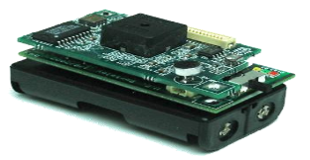
\includegraphics[width=7cm,height=3.7cm]{Chap1/chap1.png}
\end{center}


Les réseaux de capteurs utilisent un très grand nombre de ces capteurs, pour former un réseau sans infrastructure établie. Chaque capteur relayant l'information sur sa propre zone de couverture, le réseau se trouve entièrement couvert.

\begin{center}
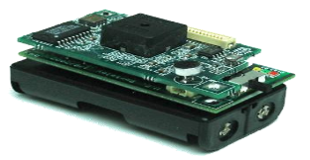
\includegraphics[width=7cm,height=3.7cm]{Chap1/chap1.png}
\end{center}



\cleardoublepage

\addcontentsline{toc}{chapter}{\numberline{}Optimisation combinatoire et méthodes de résolutions }
\addtocontents{lof}{\textbf{Optimisation combinatoire et méthodes de résolutions }}

\setcounter{chapter}{2}
\setcounter{section}{0}
\setcounter{figure}{0}

\begin{center}
	\Huge\textbf{Optimisation combinatoire et méthodes de résolutions }
\end{center}

\section{Introduction}
L’optimisation combinatoire occupe une place très importante dans divers domaines. En effet, elle définit un cadre formel pour de nombreux problèmes dans plusieurs secteurs tels que l’industrie, la finance ou tout simplement les problèmes de la vie quotidienne.
La solution optimale à un problème d’optimisation ne peut que très rarement être déterminée en un temps polynomial. Il est donc souvent nécessaire de trouver des modes de résolution qui fournissent une solution de bonne qualité dans un laps de temps raisonnable. Il existe donc des méthodes de résolution exactes qui sont caractérisées par le fait qu’elles permettent d’obtenir une ou plusieurs solutions optimales, ainsi que des méthodes de résolution approchées qui fournissent des solutions de bonne qualité (proches de l’optimal mais sans garantie d’optimalité) et dont le temps de résolution sera plus faible \cite{zidi2006systeme}.

Ce chapitre sera structuré comme suit : d’abord, nous allons présenter brièvement les techniques de routage dans les RCSFs, par la suite nous nous pencherons sur les techniques d’optimisation combinatoire, exactes et approchées surtout, pour la résolution des problèmes NP-Difficiles. Tout ceci sera clôturé par une conclusion.

Depuis une vingtaine d’années, les heuristiques les plus populaires, et également les plus efficaces, sont des techniques générales, appelées méta-heuristiques, qu’il s’agit de l’adapter à chaque problème dont sa complexité est NP-hard. Dans ce chapitre, nous allons définir c’est quoi une méta-heuristique, la classification des méthodes utilisées dans les méta-heuristiques. 

\section{Techniques d’optimisation combinatoire:}
L’importance de l’optimisation combinatoire se justifie d’un coté par la grande difficulté des problèmes d’optimisation et d’un autre coté par la quantité innombrable d’applications pratiques pouvant être formulées sous la forme de tels problèmes. En effet, ces derniers sont souvent faciles à formaliser ou à exprimer, mais peuvent toutefois, être très difficiles à résoudre. Néanmoins, la plupart d’entre eux ne possèdent pas à ce jour de solution efficace valable pour toutes les données. \cite{hao1999metaheuristiques}

Un problème d’optimisation combinatoire est exprimé sous forme d’une fonction objectif qui est à maximiser, ou à minimiser, selon le type de problème traité. La résolution d’un tel problème revient à chercher la meilleure solution (optimum global) dans l’ensemble des solutions réalisables, sans pour autant être coincé dans des solutions intermédiaires (optimum locaux), propres à un sous-espace de recherche (voir Figure \ref{fig:DOGOL}).

\begin{figure}[H]
	\centering
	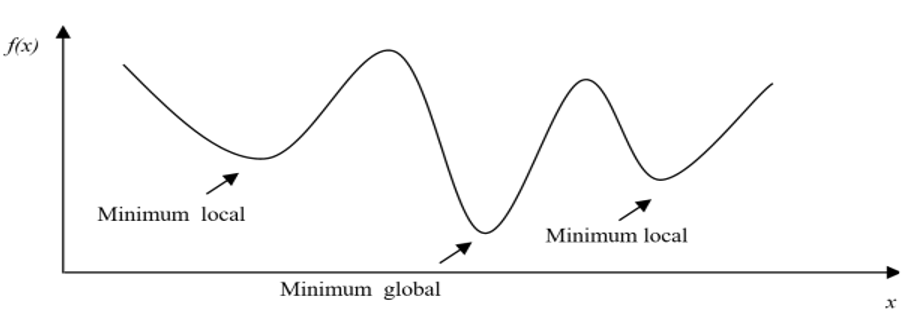
\includegraphics[width=15cm,height=5cm]{Chap2/1.png}
	\caption{Différence entre un optimum global et des optima locaux}
	\label{fig:DOGOL}
\end{figure}

L’élégance des problèmes d’optimisation combinatoire réside dans la possibilité de les modéliser en problèmes de la théorie des graphes et ainsi profiter des outils de cette dernière.

\begin{figure}[H]
	\centering
	\includegraphics[width=15cm,height=13cm]{Chap2/2.png}
	\caption{Classification des méthodes de résolution d’optimisation combinatoire}
	\label{fig:CMROC}
\end{figure}

De nombreuses méthodes de résolution ont été développées par la communauté scientifique (recherche opérationnelle, intelligence artificielle).

Ces méthodes sont divisées en deux grandes catégories : les méthodes exactes basées sur l’énumération de toutes les solutions réalisables, chose qui garantie la complétude de la résolution, et les méthodes approchées qui perdent en exactitude pour gagner en efficacité \cite{park2007dominating} . La figure \ref{fig:CMROC} illustre un schéma résumant la classification des différentes méthodes discutées le long du chapitre.

\subsection{Méthodes exacte}
Ces méthodes sont dites complètes ou exactes car elles permettent de trouver la solution optimale pour une instance de taille finie dans un temps limité et de prouver son optimalité \cite{puchinger2005combining} . Ces méthodes se basent généralement sur sur une recherche complètes de l’espace des combinaisons afin de trouver une solution optimale.\\
Les algorithmes exacts les plus réussis dans la littérature: 


\begin{enumerate}[label=\alph*)]
	\item \textbf{La méthode séparation et évaluation (Branch and Bound):} elle repose sur une méthode arborescente de recherche d’une solution optimale par séparations et évaluations. Le branch-and-bound est basé sur trois axes principaux: L’évaluation, la séparation, la stratégie de parcours.
	\begin{itemize}
		\item \textbf{L’évaluation: } permet de réduire l’espace de recherche en éliminant quelques sous ensembles qui ne contiennent pas la solution optimale.
		\item \textbf{La séparation: } a pour but de choisir un sous-problème parmi tous ceux non encore choisis. Elle associe donc à chacun une évaluation (valeur minimale) de toutes les solutions le constituant. Un sous-problème peut être supprimé dans le cas où son évaluation est supérieure à la meilleure solution connue.
		\item \textbf{La stratégie de parcours: } c’est le processus qui permet de parcourir l’ensemble des sommets et de déterminer lequel sera séparé.
	\end{itemize}
	\item \textbf{Les méthodes de coupes planes (Cutting-Plane): }type de problème à résoudre. Néanmoins, ce sont des méthodes destinées à trouver des solutions entières pour des problèmes d’optimisation combinatoire qui sont représentés sous forme d’un programme linéaire \cite{schrijver1986theory} .
	\item \textbf{La méthode (Branch and Cut): }face aux problèmes difficiles. De même que l’algorithme du "Branch and Bound". Pour cela la méthode "Branch and Cut" qui conjugue l’effort des deux algorithmes précédemment cités est utilisée \cite{padberg1991branch,padberg1987optimization} .
\end{enumerate}

\subsection{Les méthodes approchées:}
Ces méthodes s’appliquent sur tous les problèmes peut importe leurs complexités et vise à trouver une solution admissible en un temps raisonnable, mais ne garantissent pas  l’optimalité d’un solution. En outre, elles ont démontré leurs robustesses et efficacités face à plusieurs problèmes d’optimisation combinatoires. Elles englobent deux classes : Heuristiques et Méta- heuristiques:
\subsubsection{Heuristiques:}
Les heuristiques sont des règles empiriques simples basées sur l'expérience, ne fournissant pas nécessairement une solution optimale. L’avantage d’utiliser une heuristique réside dans l’efficacité de calculer une solution approchée dans un temps raisonnable et ainsi accélérer le processus de résolution exact, qui peut s’avérer long pour des problèmes à large échelle. Généralement, une heuristique n’offre aucune garantie quant à la qualité de la solution. On peut distinguer une classe d’heuristique qui est les méthodes constructives.

	Les approches constructives construisent une ou plusieurs combinaisons de façon incrémentale, c’est-à-dire, en partant d’une solution initiale vide, et à chaque itération, une variable est choisie (selon une heuristique ou aléatoirement) jusqu’à l’obtention d’une combinaison complète. c'est pour cela ces approches sont dites “basées sur les modèles” dans \cite{zlochin2004model} .\\
Il existe différentes stratégies pour choisir les composants à ajouter à chaque itération, les plus connues étant les stratégies gloutonnes. Ces stratégies consistent à construire une solution pas à pas
sans retour arrière, en prenant à chaque étape la solution qui semble la meilleure localement (selon une heuristique), en espérant obtenir une solution optimale. 

\subsubsection{Meta-Heuristiques:}
Une Méta-heuristique peut être définie comme une méthode algorithmique capable de guider et d’orienter le processus de recherche dans un espace de solution (souvent très grand) à des régions riches en solutions optimales dans le but de trouver des solutions, peut-être pas toujours optimales, en tout cas très proches de l’optimum, en un temps raisonnable.

\subsubsection{Méthodes de voisinage (A solution unique):}
Les méthodes de voisinage se basent sur la notion de voisinage. Elle a plusieurs méthodes chacune débute avec une configuration initiale, et réalise ensuite un processus itératif qui consiste à remplacer la configuration courante par l'un de ses voisins en tenant compte de la fonction de coût. Ce processus s'arrête et retourne la meilleure configuration trouvée quand la condition d'arrêt est réalisée. Cette condition d'arrêt concerne généralement une limite pour le nombre d'itérations, le temps d’exécution ou un objectif à réaliser. Présentant quelques méthodes:

\begin{enumerate}[label=\alph*)]
	\item \textbf{Recuit simulé: } La recherche recuit simulé a été introduite en 1983 par Kirkpatrick et al. \cite{kirkpatrick1983optimization}. Cette méthode originale est basée sur les travaux bien antérieurs de Metropolis et al. \cite{metropolis1953equation} et elle est considérée comme la plus ancienne méta-heuristique.\\
Le principe de fonctionnement s’inspire d’un processus d’amélioration de la qualité d’un métal solide par recherche d’un état d’énergie minimum correspondant à une structure stable de ce métal. L’état optimal correspondrait à une structure moléculaire régulière parfaite. En partant d’une température élevée où le métal serait liquide, on refroidit le métal progressivement en tentant de trouver le meilleur équilibre thermodynamique.\\
La popularité du recuit simulé a été incontestable pendant des années. D’abord cette méthode est facile à implémenter et elle a permis de résoudre de nombreux problèmes NP-difficiles \cite{bonomi1984n,vidal1993applied}.\\
\begin{figure}[h]
	\centering
	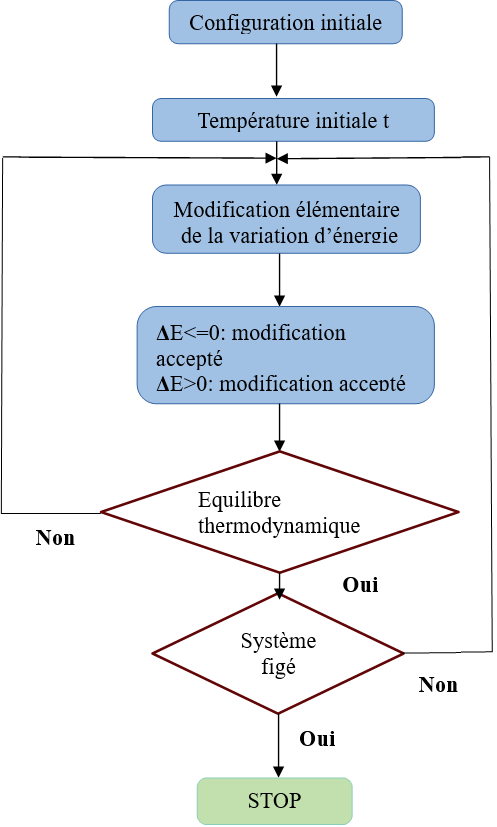
\includegraphics[width=9cm,height=10cm]{Chap2/3.png}
	\caption{Organigramme  illustrant le fonctionnement  de la recherche Recuit simulé}
	\label{fig:OIFRR}
\end{figure}

\begin{algorithm}[H]
\caption{Recuit simulé }
%\KwData{this text}
%\KwResult{la meilleure combinaison ayant appartenu à la population }
\SetAlgoLined
\DontPrintSemicolon
$ t \gets 0 $ , Initialiser la température T en fonction du schéma de refroidissement \;
$ s\gets s_0 $ , une solution initiale \;
$ Best \gets S $ \;
\While{(Best est la meilleure) $\cap$ (nombre iter=max) $\cap$ ($ t \leq 0 $)}{
  $ r \gets s’$ où $s’ \in N(s)$ \;
  $ \rho \gets random(0.1)$ \;
  $ \triangle E = f(r)-f(s) $  \;
  \If{ $ f(r) < f(s)  \cup \rho < e^{-\triangle E/t }$ }{
	$ s \gets r $ \;
   }
  \If{f(s)<f(Best)}{
	$ Best \gets s$ \;
   }
   Décrémenter le t \;
 }
\end{algorithm}


	\item \textbf{Recherche tabou: } La méthode de recherche avec tabous, ou simplement recherche tabou (TS :Tabu Search) a été formalisée par Fred Glover en 1986 \cite{glover1986future} . Elle utilise explicitement l’historique de la recherche, à la fois pour échapper aux minimaux locaux et pour mettre en œuvre une stratégie d’exploration. Sa principale caractéristique est en effet basée sur  l’utilisation de mécanismes inspirés de la mémoire humaine. A l'inverse du recuit simulé qui génère de manière aléatoire une seule solution voisine s’ \( \in N(s) \) à chaque itération, la recherche tabou examine un échantillonnage de solutions de \( N(s) \) et retient la meilleure s’ même si s’ est plus mauvaise que s. La recherche tabou ne s'arrête donc pas au premier optimum trouvé.\\
La méthode TS utilise une liste tabou, qui mémorise les dernières solutions rencontrées (ou des caractéristiques de solutions) vers lesquelles il est interdit de se déplacer. Ce procédé simple de mémoire permet de choisir le meilleur voisin non tabou, même si celui-ci dégrade la fonction-objectif f. Cependant, dans certains cas, les interdictions occasionnées par la liste tabou peuvent être jugées trop radicales. En effet, on risque d’éliminer (en les rendant tabous), certains mouvements particulièrement utiles. Pour éviter cela, on incorpore dans l’algorithme un mécanisme d’aspiration
qui détermine des critères selon lesquels un mouvement, bien que tabou, peut quand même être
accepté, s’il permet d’obtenir une meilleure solution que toutes celles déjà parcourues.\\
La taille de la liste tabou contrôle la mémoire du processus de recherche. Pour favoriser l’intensification, il suffit de diminuer la taille de la liste tabou. En revanche, augmenter la taille de la liste tabou, forcera le processus de recherche à explorer des régions plus vastes, favorisant ainsi la diversification. La taille de la liste tabou peut être modifiée au cours de la recherche \cite{battiti1994reactive}.\\
Une autre amélioration intéressante de la TS est l’utilisation de structure de mémoire à moyen et à long terme afin d’approfondir les notions d’intensification et de diversification.\\
\begin{figure}[H]
	\centering
	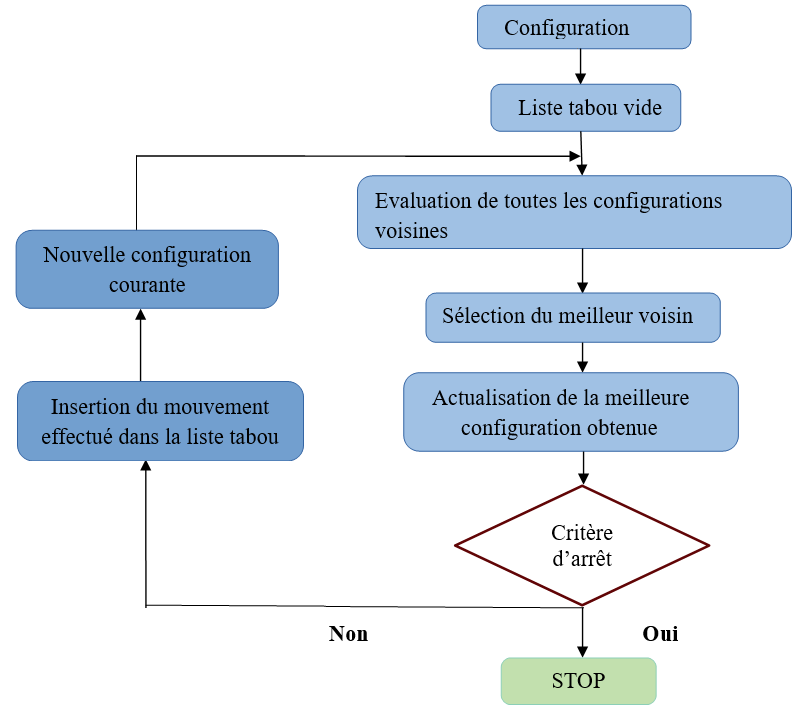
\includegraphics[width=12cm,height=8cm]{Chap2/4.png}
	\caption{Organigramme illustrant le  Fonctionnement de l’algorithme TS}
	\label{fig:OIFA}
\end{figure}
\begin{algorithm}[h!]
\caption{Recherche Taboue}
\SetAlgoLined
\DontPrintSemicolon
$ l \gets longueur maximale de la liste taboue $  \;
$ n \gets number of tweaks desired to sample the gradient$ \;
$ S \gets solution initial $ \;
$ Best \gets S $ \;
$ L \gets \{\} $ \;
Insérer s dans L \;

\While{(Best est la meilleure) $\cap$ (nombre iter=max)}{
  \If{ $ longueur(L) > l $ }{
    Défiler un élément de la liste L \;
   }
   $r \gets r’$ où  $r’ \in N(s)$  \;  
   \For{$i\gets1$ \KwTo $N-1$ }{
     $w \gets w’$ où  $w’ \in N(s)$  \;
     \If{$ w \notin L  \cap ( f(w)<f(r) \cup r \in L ) $ }{
		$ e \gets w $ \;
		\If{$ r \notin L  \cap f(r)<f(s) $}{
           $ s \gets r $ \;
           Enfiler r dans L \;
		}
		\If{$f(s)<f(Best)$}{
			$ Best \gets s $			
		}
     }
   }
 }

\end{algorithm}



	
	\item \textbf{Recherche locale : } Pour cette méthode de recherche il suffit de tester itérativement de nouvelles solutions potentielles dans la région de la solution courante, et de prendre la meilleure dans le voisinage. La méthode est une généralisation de la méthode de la descente de gradient elle consiste à partir d’une solution s à choisir une solution s’ dans un voisinage de s, noté N(s). La nouvelle solution choisie est meilleure que la précédente sous la fonction objective. Cela nous permet d’explorer l’espace des combinaisons  de proche en proche, en partant d’une combinaison initiale et en sélectionnant à chaque itération une combinaison voisine de la combinaison courante, obtenue en lui appliquant une transformation élémentaire jusqu’à la convergence à un optimum local. L’algorithme  décrivant le principe général de la recherche locale:\\

\begin{algorithm}[H]
\caption{Recherche Local}
\SetAlgoLined
\DontPrintSemicolon

$ s \gets solution initial $ \;
\While{ (Best est la meilleure) $\cap$ (nombre iter=max) }{
	$ r \gets s’$ où $s’ \in N(s)$ \;
	\If{ $f(r) < f(s)$ }{
		$ s \gets r $  \;		
	}
}

\end{algorithm}
	
	
	\item \textbf{Recherche à voisinages variables(VNS):} La recherche à voisinage variable (VNS : Variable neighborhood search) est une méta-heuristique proposée par Hansen et Mladenovic en 1997 [28,29]. Elle est basée sur le principe de changement systématique de voisinage durant la recherche (la performance des méthodes de descente).  La procédure de VNS se compose de trois étapes : perturbation (shaking), recherche locale et déplacement. Cet algorithme est efficace si les structures de voisinage sont complémentaires en ce sens qu’un minimum local pour un voisinage n’en n’est pas nécessairement un pour un autre, ce qui veut dire simplement d’utiliser plusieurs voisinages successifs quand on se trouve bloqué dans un minimum local.\\
	
\begin{algorithm}[H]
\caption{Recherche à voisinages variables (VNS)}
\SetAlgoLined
\DontPrintSemicolon

$ s \gets solution initial $ \;
\Repeat{$ K = K_{Max} $}{
	générer $s’$ ,tel que $s’ \in N(s)$ \;
	$s'' \gets Appel$(Recherche Locale) \;
	\eIf{$f(s'') < f(s)$}{
		$ s \gets s'' $ \;
		$ K \gets 1 $ \;		
	}{
		$ K = K + 1 $ \;
	}
}
	

\end{algorithm}

	
\end{enumerate}



\subsubsection{Méthodes évolutives (A population):}
Depuis le début des années 90, une autre famille d’ heuristiques est devenue très populaire : les Méthodes Évolutives \cite{hertz2000framework} , s’inspirant de la théorie de l’évolution «darwinienne»  tels que le croisement, la mutation et la sélection pour résoudre des problèmes divers. Contrairement à la Recherche Locale qui tente d’ améliorer itérativement une solution courante. Les Méthodes Évolutives travaillent sur une population de solutions en appliquant un processus cyclique composé d’ une phase de coopération et d’ une phase d’adaptation individuelle qui se succèdent à tour de rôle. Dans la phase de coopération, les solutions de la population courante sont comparées entre elles, puis combinées, dans le but de produire de nouvelles solutions qui héritent des bons aspects de chaque membre de la population. Dans la phase d’adaptation individuelle, chaque solution dans la population peut évoluer de manière indépendante. On peut utiliser le même type de critère d’ arrêt que dans la Recherche Locale, ou alors on peut décider de stopper une Méthode Évolutive dès que les solutions dans la population sont jugées trop similaires. Une description générale des Méthodes Évolutives est donnée ci-dessous:

\begin{figure}[H]
	\centering
	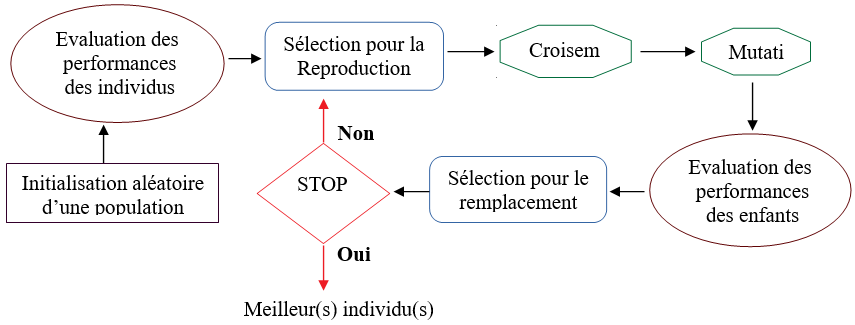
\includegraphics[width=15cm,height=7cm]{Chap2/5.png}
	\caption{Principe d’un algorithme évolutionnaire (EA) \cite{dreo2003metaheuristiques}.}
	\label{fig:PAEEA}
\end{figure}

Le terme Evolutionary Computation englobe une classe assez large de méta-heuristiques qui ont été développés au début des années soixante, telles que les algorithmes génétiques \cite{holland1975adaptation}, les stratégies d’évolution \cite{rechenberg1973evolutionsstrategie} , la programmation évolutive \cite{fogel1966artificial}, et la programmation génétique \cite{koza1992genetic}

\begin{enumerate}[label=\alph*)]
	\item \textbf{Algorithmes génétiques(AG):} développées par J. Holland en 1975 \cite{holland1975adaptation} comme outils de modélisation de l’adaptation et qui travaillent dans un espace de chaînes de bits. Elles ont été largement utilisé et développé par [ Moscato en 1989 \cite{moscato1989evolution} ]. Cette classe s’inspire de la théorie de l’évolution et des règles de la génétique qui expliquent la capacité des espèces de s’adapter à leurs environnement à l’ aide de l’ opérateur de mutation, alors que l’ échange d’information est gouverné par un opérateur de reproduction et un opérateur de combinaison (ou croisement). L’algorithme ci-dessous décrit ce principe général, dont les principales étapes sont détaillées ci-après.\\

\begin{figure}[H]
	\centering
	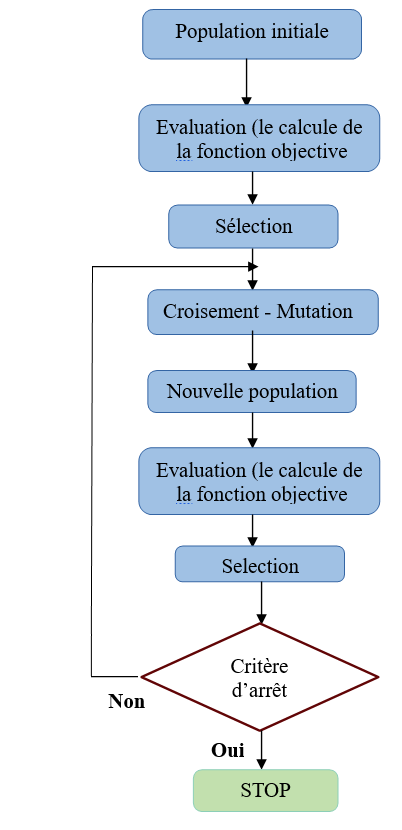
\includegraphics[width=9cm,height=10cm]{Chap2/6.png}
	\caption{Organigramme d’un algorithme génétique}
	\label{fig:OAG}
\end{figure}

\begin{algorithm}[H]
\caption{Algorithme génétique}
\KwResult{la meilleure combinaison ayant appartenu à la population }
\SetAlgoLined
\DontPrintSemicolon

Initialiser la population avec un ensemble de combinaisons de E \;
\While{critères d’arrêt non atteints}{
	Sélectionner des combinaisons de la population \;
	Créer de nouvelles combinaisons par croisement et mutation \;
	Mettre à jour la population  \;
}

\end{algorithm}

	
\begin{itemize}
	\item \textbf{Initialisation de la population: }en général, la population initiale est générée de façon aléatoire, selon une distribution uniforme assurant une bonne diversité des combinaisons. Une solution initiale est de bonne qualité, celle qui nous permet de converger vers un optimum global dans le plus court délai possible.
	
Il est à noter que cette méthode est utilisée dans toutes les méta-heuristiques avec population.

	\item \textbf{Sélection: } cette étape consiste à choisir les combinaisons de la population qui seront ensuite croisées et mutées. Il s’agit là de favoriser la sélection des meilleures combinaisons, tout en laissant une petite chance aux moins bonnes combinaisons. Il existe de nombreuses façons de procéder à cette étape de sélection. Par exemple, la sélection par tournoi consiste à choisir aléatoirement deux combinaisons et à sélectionner la meilleure des deux (ou bien à sélectionner une des deux selon une probabilité dépendant de la fonction objectif).
	
	\item \textbf{Croisement:} est une opération de diversification. cette opération consiste à générer de nouvelles combinaisons, à partir des deux individus sélectionnés. Là encore, il existe de nombreux opérateurs de croisement. Une méthode simple consiste à choisir aléatoirement un point de croisement, à couper chaque combinaison parente en ce point, puis à reformer deux enfants en échangeant les parties composant les parents de part et d’autre du point de croisement.
	
	\item \textbf{Mutation: } cette opération consiste à modifier de façon aléatoire certains composants des combinaisons obtenues par croisement.
	
	\item \textbf{Mise à jour de la population: } cette étape consiste à remplacer certaines combinaisons de la génération précédente par certaines combinaisons issues des opérations de croisement et de mutation, formant de la sorte une nouvelle génération. Là encore, il existe différentes stratégies de remplacement, favorisant plus ou moins la diversité, et plus ou moins élitistes. On peut par exemple choisir de ne garder que les meilleurs individus, qu’ils soient issus de la nouvelle génération ou de l’ancienne, ou bien ne garder que les individus de la nouvelle génération, indépendamment de leur qualité.
	
	\item \textbf{Critères d’arrêt: } le processus d’évolution est itéré, de génération en génération, jusqu’à ce qu’une combinaison de qualité suffisante soit générée, ou bien jusqu’à ce qu’une limite de temps soit atteinte. On peut également utiliser des indicateurs de diversité (comme par exemple le taux de ré-échantillonnage ou la distance pair-à-pair) pour arrêter le processus lorsque la population est devenue trop uniforme. On peut aussi limiter le nombre d’itération possible ou encore les probabilités d’application des opérateurs de croisement et de 
mutation.
 
\end{itemize}	

	
	\item \textbf{L’optimisation des colonies de fourmis (ACO): }est une technique d’intelligence artificielle qui s'inspire du comportement intelligent des fourmis lors de la recherche de nourriture. Cette méta-heuristique permet de trouver des solutions de haute qualité aux problèmes d’optimisation combinatoire. 

En raison de leur comportement de recherche de nourriture, les fourmis trouvent les chemins les plus courts entre leur nid et leur source de nourriture, en déposant sur la terre une substance chimique appelée phéromone. Cela forme une traînée de phéromone qui est utilisée pour la communication stigmergique. La présence d'une telle phéromone sur les trajectoires affecte la prise de décision des fourmis concernant les trajectoires choisies par elles. Les fourmis sélectionnent de manière probabiliste les chemins marqués par de fortes concentrations de phéromones ce qui permet aux fourmis de trouver le chemin le plus court vers la source de nourriture.\\


\begin{algorithm}[H]
\caption{L’optimisation des colonies de fourmis (ACO)}
\KwResult{la meilleure solution trouvée}
\SetAlgoLined
\DontPrintSemicolon

Initialisation : initialisation de phéromones et les paramètre avec des valeurs constantes \;
Construction de la solution initiale \;
\While{condition d’arrêt non atteinte }{
	\While{nombre de fourmis non atteint}{
		Construction d’une solution selon la concentration de phéromone \;
		Mise à jour en ligne de  la table des phéromones \;
	}
	\If{la meilleure solution trouvée par l’itération courante est meilleure que celles des 	itérations précédente}{
		Mise à jour de l a solution courante \;
	}
	Mise à jour hors ligne de  la table des phéromones \;	
}

\end{algorithm}

\begin{itemize}
	\item \textbf{Solution initiale:} en général, la solution initiale est générée de façon aléatoire.Une solution est composée de plusieurs attributs définis selon la nature du problème.
	
	\item \textbf{Initialisation de la table de phéromone:} la table de phéromone contient  la concentration de phéromone pour tous les attributs possible d’une solution. Au départ tous les attributs ont une même concentration de phéromone. 
	
	\item \textbf{Mise à jour de phéromone:}
		\begin{itemize}
			\item \textbf{En ligne:} les attributs communs entre la solution courante et la meilleure solution vont être favoriser par une valeur constante supplémentaire.
			\item \textbf{Hors ligne:} les attributs appartenant à la meilleure solution vont être favoriser par la valeur constante. 
		\end{itemize}
\end{itemize}
	
	\item \textbf{L’algorithme à base de biogéographie (BBO)} BBO est un algorithme inspiré de la biogéographie, qui étudie la répartition géographique des organismes biologiques.

Tout comme GA et PSO qui sont basés sur la biologie, BBO est un algorithme basé sur une population dans lequel chaque population de solutions candidates est utilisée dans la procédure de recherche d’un optima global. BBO présente certaines caractéristiques communes avec l’algorithme d'optimisation, le GA. En GA, un individu de la population s'appelle un chromosome et a sa propre valeur de condition physique. De même, dans BBO, chaque individu est qualifié d'habitat et a son indice de qualité de l'habitat (HSI) pour évaluer sa qualité en tant que solution. Comme nous avons affaire à un problème de minimisation, un habitat à faible indice de sécurité d'impact représente une bonne solution et un habitat à haut indice de faiblesse est plutôt une solution médiocre. Chaque chromosome de GA est constitué de gènes, tandis que, pour BBO, chaque habitat est caractérisé par des variables d'indice de pertinence (SIV). L'AG compte deux opérateurs principaux: le croisement et la mutation. Pendant ce temps, chez BBO, les principaux opérateurs sont la migration et la mutation. L'opérateur de migration est composé d'émigration et d'immigration. Il est utilisé pour améliorer et faire évoluer les habitats (solutions au problème d'optimisation) de la population. Les fonctionnalités de solution (SIV) émigrent d'habitats à faible HSI (habitats d'émigration) vers des habitats à haut HSI (habitats d'immigration). Il existe différentes alternatives pour les processus de migration et de mutation de BBO. La manière dont nous implémentons ces deux opérateurs est expliquée en détail dans le prochain chapitre. \\


\begin{algorithm}[H]
\caption{L’algorithme à base de biogéographie (BBO)}
\KwResult{la meilleure solution ayant appartenu à la population }
\SetAlgoLined
\DontPrintSemicolon

Générer aléatoirement un ensemble de solutions initiales (îles) \;
\While{le critère d’arrêt n’est pas atteint}{
	Évaluer la fitness (HSI) de chaque solution \;
	Calculer le nombre d’espèce $S$, le taux d’immigration $\lambda$ et d’émigration $\mu$ pour chaque solution \;
	\textbf{Migration}  \;
	\textbf{Mutation} : muter les individus au taux de mutation \;
	Remplacement de la population par les descendants \;
	Implémenter l’\textbf{élitisme}  \;
}

\end{algorithm}

Dans le processus de migration (algorithme \ref{alg:MIGRATION}), quand une solution est sélectionnée pour être changée, nous utilisons le taux d'immigration $\lambda$ pour décider si un SIV sera changé. Dans ce cas, nous utilisons le taux d'émigration $\mu$ pour décider quelle bonne solution migrera son SIV.\\
Cette algorithme  sera suivit d’une figure qui ellustre le fonctionnement de ce processus (figure \ref{fig:PMBBO}) \\

\begin{algorithm}[H]
\label{alg:MIGRATION}
\caption{migration}
\SetAlgoLined
\DontPrintSemicolon

\For{$i\gets1$ \KwTo $N$}{
	Utiliser $\lambda_i$ pour décider, de manière probabiliste, d’immigrer à $X_i$ \;
	\If{$rand(0,1) < \lambda_i $}{
		\For{$j \gets 1$ \KwTo $N$}{
			Sélectionner un habitat d’émigration $X_j$ avec une probabilité $\alpha \mu_j $ \;
			\If{$rand(0,1) < \mu_j$}{
				Remplacer une variable de décision (SIV) choisie aléatoirement dans par la variable correspondante dans $X_j$ \;				
			}
		}
	}
}

\end{algorithm}



Où : \\
$\lambda_k$ : est le taux d'immigration dans un habitat de k espèces \\
$\mu_k $ : est le taux d'émigration dans un habitat de k espèces. \\
$E$ : est le taux maximal d'émigration.\\
$I$ : est le taux maximal d'immigration. Supposons que nous avons une population de solutions candidates à un problème, représentées par des vecteurs (habitats $H_i , i = 1...n $)\\
$N$ : est le nombre maximum d'espèces.\\
$k$ : est le nombre d'espèces.\\
\textbf{Mutation:} c’est le même principe qui est utilié pour l’algorithme génétique.\\
\textbf{Elitisme:} cette méthode consiste à garder les meilleurs individus de chaque population. La méthode d’élitisme risque d’élaguer les individus de mauvaise qualité mais ça n’empêche pas de produire une population avec des résultats meilleurs ou au moins de créer des individus qui auront pu apporter de quoi créer de très bonnes solution dans les populations suivantes. \\

\begin{figure}[H]
	\centering
	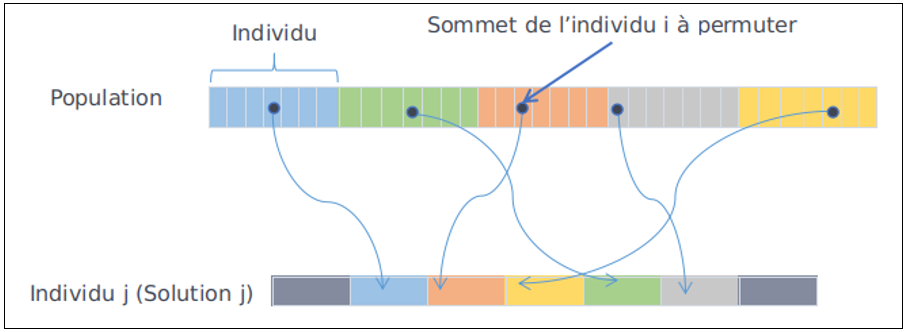
\includegraphics[width=15cm,height=6cm]{Chap2/7.png}
	\caption{processus de migration de BBO}
	\label{fig:PMBBO}
\end{figure}	
	
	\item \textbf{Algorithmes mémétiques (algorithme de colonies de fourmis \& d’essaim de particules) : }
Le terme «algorithmes mémétiques»  est apparu pour la première fois dans [38], introduit par Moscato en 1986. L’idée principale de ce genre d’algorithme est de rendre plus agressif un algorithme génétique par l’ajout d’une recherche locale en plus de la mutation.

La faible vitesse de convergence est la première observation provenant de l’implémentation de l’algorithme génétique. Pour cet effet Moscoto a pensé d’ajouter une recherche locale  qui peut être une méthode de descente ou une recherche locale plus évoluée (recuit simulé ou recherche tabou par exemple). Cette recherche locale sera appliquée à tout nouvel individu obtenu au cours de la recherche.

D’une vue globale, l’application de cette simple modification n’influe en rien sur le comportement de l’algorithme, mais  cela peut apporter de profondes changement en ce dernier. Après avoir créé un nouvel individu à partir de deux parents sélectionnés, on applique une recherche locale et sous certaines conditions on applique un opérateur de mutation à cet individu. Les conditions peuvent être une certaine probabilité. Il est aussi possible d’ajouter un critère d’aspiration ou d’autres techniques plus évoluées à cet endroit.\\


\begin{algorithm}[H]
\caption{Simple Algorithme mémétique}
\KwResult{la meilleure solution ayant appartenu à la population }
\SetAlgoLined
\DontPrintSemicolon

Initialisation : générer une population initiale $P$ de solutions de taille $| P | = n$  \;
\Repeat{critère d'arrêt satisfait}{
	Sélection: choisissez 2 solutions s et $s’$ avec la technique volue \;
	Croisement: combinez les solutions parentes s et $s’$ pour former une solution enfant $y$ \;
	Recherche locale: appliquer une procédure de recherche locale sur y sous certaines conditions \;
	Mutation: appliquer un opérateur de mutation sur y dans des conditions \;
	Choisir un individu y’ à remplacer dans la population \;
	remplacer y’ par y dans la population \;	
}

\end{algorithm}

\begin{figure}[H]
	\centering
	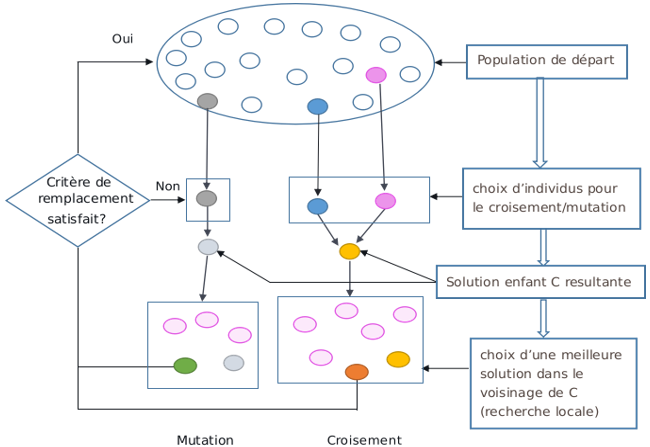
\includegraphics[width=15cm,height=10cm]{Chap2/8.png}
	\caption{Schéma explicatif d’un algorithme mémétique}
	\label{fig:SEAM}
\end{figure}
	
\end{enumerate}


\section{Conclusion}
Nous avons présenté dans ce chapitre l’état de l’art des méta-heuristiques pour l’optimisation des problèmes Np-difficile. Plus de détails sur le problème de l’arbre dominant qui en est un, ainsi que les méthodes utilisées pour sa résolution seront mis au clair dans le prochain chapitre.



\cleardoublepage

\addcontentsline{toc}{chapter}{\numberline{}3eme chapiter}
\addtocontents{lof}{\textbf{Chapter A3}}

\setcounter{chapter}{3}
\setcounter{section}{0}
\setcounter{figure}{0}

\begin{center}
	\Huge\textbf{3eme chapter}
\end{center}

\section{Introduction}
L’optimisation combinatoire occupe une place très importante dans divers domaines. En effet, elle définit un cadre formel pour de nombreux problèmes dans plusieurs secteurs tels que l’industrie, la finance ou tout simplement les problèmes de la vie quotidienne.
La solution optimale à un problème d’optimisation ne peut que très rarement être déterminée en un temps polynomial. Il est donc souvent nécessaire de trouver des modes de résolution qui fournissent une solution de bonne qualité dans un laps de temps raisonnable. Il existe donc des méthodes de résolution exactes qui sont caractérisées par le fait qu’elles permettent d’obtenir une ou plusieurs solutions optimales, ainsi que des méthodes de résolution approchées qui fournissent des solutions de bonne qualité (proches de l’optimal mais sans garantie d’optimalité) et dont le temps de résolution sera plus faible \cite{zidi2006systeme}.

Ce chapitre sera structuré comme suit : d’abord, nous allons présenter brièvement les techniques de routage dans les RCSFs, par la suite nous nous pencherons sur les techniques d’optimisation combinatoire, exactes et approchées surtout, pour la résolution des problèmes NP-Difficiles. Tout ceci sera clôturé par une conclusion.\\
Depuis une vingtaine d’années, les heuristiques les plus populaires, et également les plus efficaces, sont des techniques générales, appelées méta-heuristiques, qu’il s’agit de l’adapter à chaque problème dont sa complexité est NP-hard. Dans ce chapitre, nous allons définir c’est quoi une méta-heuristique, la classification des méthodes utilisées dans les méta-heuristiques. 

\section{Techniques d’optimisation combinatoire:}
L’importance de l’optimisation combinatoire se justifie d’un coté par la grande difficulté des problèmes d’optimisation et d’un autre coté par la quantité innombrable d’applications pratiques pouvant être formulées sous la forme de tels problèmes. En effet, ces derniers sont souvent faciles à formaliser ou à exprimer, mais peuvent toutefois, être très difficiles à résoudre. Néanmoins, la plupart d’entre eux ne possèdent pas à ce jour de solution efficace valable pour toutes les données. \cite{hao1999metaheuristiques}

Un problème d’optimisation combinatoire est exprimé sous forme d’une fonction objectif ; qui est à maximiser, ou à minimiser, selon le type de problème traité. La résolution d’un tel problème revient à chercher la meilleure solution (optimum global) dans l’ensemble des solutions réalisables, sans pour autant être coincé dans des solutions intermédiaires (optimum locaux), propres à un sous-espace de recherche (voir Figure 3.1).

\begin{figure}[h]
	\centering
	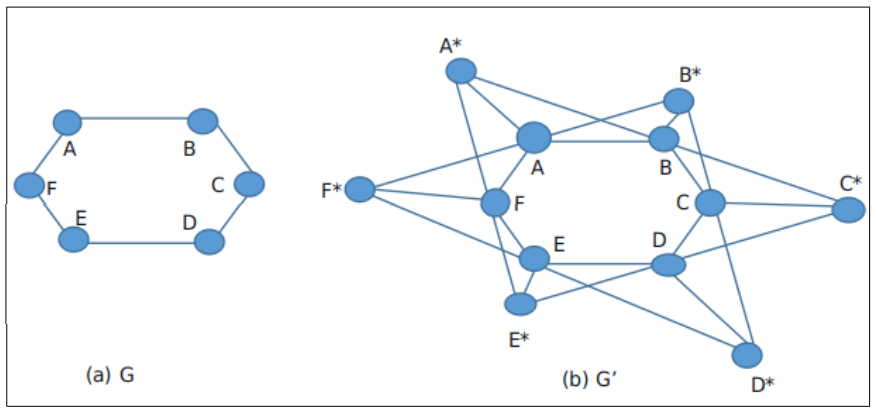
\includegraphics[width=15cm,height=5cm]{Chap3/1.png}
	\caption{Différence entre un optimum global et des optima locaux}
	\label{fig:CSF}
\end{figure}

L’élégance des problèmes d’optimisation combinatoire réside dans la possibilité de les modéliser en problèmes de la théorie des graphes et ainsi profiter des outils de cette dernière.

\begin{figure}[H]
	\centering
	\includegraphics[width=15cm,height=13cm]{Chap3/2.png}
	\caption{Classification des méthodes de résolution d’optimisation combinatoire}
	\label{fig:CSF}
\end{figure}

De nombreuses méthodes de résolution ont été développées par la communauté scientifique (recherche opérationnelle, intelligence artificielle).

Ces méthodes sont divisées en deux grandes catégories : les méthodes exactes basées sur l’énumération de toutes les solutions réalisables, chose qui garantie la complétude de la résolution, et les méthodes approchées qui perdent en exactitude pour gagner en efficacité \cite{park2007dominating} . La figure 3.2 illustre un schéma résumant la classification des différentes méthodes discutées le long du chapitre.

\subsection{Méthodes exacte}
Ces méthodes sont dites complètes ou exactes car elles permettent de trouver la solution optimale pour une instance de taille finie dans un temps limité et de prouver son optimalité \cite{puchinger2005combining} . Ces méthodes se basent généralement sur sur une recherche complètes de l’espace des combinaisons afin de trouver une solution optimale.\\
Les algorithmes exacts les plus réussis dans la littérature: 


\begin{enumerate}[label=\alph*)]
	\item \textbf{La méthode séparation et évaluation (Branch and Bound):} elle repose sur une méthode arborescente de recherche d’une solution optimale par séparations et évaluations. Le branch-and-bound est basé sur trois axes principaux: L’évaluation, la séparation, la stratégie de parcours.
	\begin{itemize}
		\item \textbf{L’évaluation: } permet de réduire l’espace de recherche en éliminant quelques sous ensembles qui ne contiennent pas la solution optimale.
		\item \textbf{La séparation: } a pour but de choisir un sous-problème parmi tous ceux non encore choisis. Elle associe donc à chacun une évaluation (valeur minimale) de toutes les solutions le constituant. Un sous-problème peut être supprimé dans le cas où son évaluation est supérieure à la meilleure solution connue.
		\item \textbf{La stratégie de parcours: } c’est le processus qui permet de parcourir l’ensemble des sommets et de déterminer lequel sera séparé.
	\end{itemize}
	\item \textbf{Les méthodes de coupes planes (Cutting-Plane): }type de problème à résoudre. Néanmoins, ce sont des méthodes destinées à trouver des solutions entières pour des problèmes d’optimisation combinatoire qui sont représentés sous forme d’un programme linéaire \cite{schrijver1986theory} .
	\item \textbf{La méthode (Branch and Cut): }face aux problèmes difficiles. De même que l’algorithme du "Branch and Bound". Pour cela la méthode "Branch and Cut" qui conjugue l’effort des deux algorithmes précédemment cités est utilisée \cite{padberg1991branch,padberg1987optimization} .
\end{enumerate}

\subsection{Les méthodes approchées:}
Ces méthodes s’appliquent sur tous les problèmes peut importe leurs complexités et vise à trouver une solution admissible en un temps raisonnable, mais ne garantissent pas  l’optimalité d’un solution. En outre, elles ont démontré leurs robustesses et efficacités face à plusieurs problèmes d’optimisation combinatoires. Elles englobent deux classes : Heuristiques et Méta- heuristiques:
\subsubsection{Heuristiques:}
Les heuristiques sont des règles empiriques simples basées sur l'expérience, ne fournissant pas nécessairement une solution optimale. L’avantage d’utiliser une heuristique réside dans l’efficacité de calculer une solution approchée dans un temps raisonnable et ainsi accélérer le processus de résolution exact, qui peut s’avérer long pour des problèmes à large échelle. Généralement, une heuristique n’offre aucune garantie quant à la qualité de la solution. On peut distinguer une classe d’heuristique qui est les méthodes constructives.

	Les approches constructives construisent une ou plusieurs combinaisons de façon incrémentale, c’est-à-dire, en partant d’une solution initiale vide, et à chaque itération, une variable est choisie (selon une heuristique ou aléatoirement) jusqu’à l’obtention d’une combinaison complète. c'est pour cela ces approches sont dites “basées sur les modèles” dans \cite{zlochin2004model} .\\
Il existe différentes stratégies pour choisir les composants à ajouter à chaque itération, les plus connues étant les stratégies gloutonnes. Ces stratégies consistent à construire une solution pas à pas
sans retour arrière, en prenant à chaque étape la solution qui semble la meilleure localement (selon une heuristique), en espérant obtenir une solution optimale. 

\subsubsection{Meta-Heuristiques:}
Une Méta-heuristique peut être définie comme une méthode algorithmique capable de guider et d’orienter le processus de recherche dans un espace de solution (souvent très grand) à des régions riches en solutions optimales dans le but de trouver des solutions, peut-être pas toujours optimales, en tout cas très proches de l’optimum, en un temps raisonnable.

\subsubsection{Méthodes de voisinage (A solution unique):}
Les méthodes de voisinage se basent sur la notion de voisinage. Elle a plusieurs méthodes chacune débute avec une configuration initiale, et réalise ensuite un processus itératif qui consiste à remplacer la configuration courante par l'un de ses voisins en tenant compte de la fonction de coût. Ce processus s'arrête et retourne la meilleure configuration trouvée quand la condition d'arrêt est réalisée. Cette condition d'arrêt concerne généralement une limite pour le nombre d'itérations, le temps d’exécution ou un objectif à réaliser. Présentant quelques méthodes:

\begin{enumerate}[label=\alph*)]
	\item \textbf{Recuit simulé: } La recherche recuit simulé a été introduite en 1983 par Kirkpatrick et al.[24]. Cette méthode originale est basée sur les travaux bien antérieurs de Metropolis et al. \cite{metropolis1953equation} et elle est considérée comme la plus ancienne méta-heuristique.\\
Le principe de fonctionnement s’inspire d’un processus d’amélioration de la qualité d’un métal solide par recherche d’un état d’énergie minimum correspondant à une structure stable de ce métal. L’état optimal correspondrait à une structure moléculaire régulière parfaite. En partant d’une température élevée où le métal serait liquide, on refroidit le métal progressivement en tentant de trouver le meilleur équilibre thermodynamique.\\
La popularité du recuit simulé a été incontestable pendant des années. D’abord cette méthode est facile à implémenter et elle a permis de résoudre de nombreux problèmes NP-difficiles \cite{bonomi1984n,vidal1993applied}.

\begin{figure}[h]
	\centering
	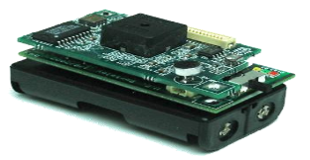
\includegraphics[width=7cm,height=3.7cm]{Chap1/1.png}
	\caption{Différence entre un optimum global et des optima locaux}
	\label{fig:CSF}
\end{figure}

\begin{algorithm}[H]
\caption{Recuit simulé }
%\KwData{this text}
%\KwResult{la meilleure combinaison ayant appartenu à la population }
\SetAlgoLined
\DontPrintSemicolon
$ t \gets 0 $ , Initialiser la température T en fonction du schéma de refroidissement \;
$ s\gets s_0 $ , une solution initiale \;
$ Best \gets S $ \;
\While{(Best est la meilleure) $\cap$ (nombre iter=max) $\cap$ ($ t \leq 0 $)}{
  $ r \gets s’$ où $s’ \in N(s)$ \;
  $ \rho \gets random(0.1)$ \;
  $ \triangle E = f(r)-f(s) $  \;
  \If{ $ f(r) < f(s)  \cup \rho < e^{-\triangle E/t }$ }{
	$ s \gets r $ \;
   }
  \If{f(s)<f(Best)}{
	$ Best \gets s$ \;
   }
   Décrémenter le t \;
 }
\end{algorithm}

	\item \textbf{Recherche tabou: } La méthode de recherche avec tabous, ou simplement recherche tabou (TS :Tabu Search) a été formalisée par Fred Glover en 1986 \cite{glover1986future} . Elle utilise explicitement l’historique de la recherche, à la fois pour échapper aux minimaux locaux et pour mettre en œuvre une stratégie d’exploration. Sa principale caractéristique est en effet basée sur  l’utilisation de mécanismes inspirés de la mémoire humaine. A l'inverse du recuit simulé qui génère de manière aléatoire une seule solution voisine s’ \( \in N(s) \) à chaque itération, la recherche tabou examine un échantillonnage de solutions de \( N(s) \) et retient la meilleure s’ même si s’ est plus mauvaise que s. La recherche tabou ne s'arrête donc pas au premier optimum trouvé. \\
	La méthode TS utilise une liste tabou, qui mémorise les dernières solutions rencontrées (ou des caractéristiques de solutions) vers lesquelles il est interdit de se déplacer. Ce procédé simple de mémoire permet de choisir le meilleur voisin non tabou, même si celui-ci dégrade la fonction-objectif f. Cependant, dans certains cas, les interdictions occasionnées par la liste tabou peuvent être jugées trop radicales. En effet, on risque d’éliminer (en les rendant tabous), certains mouvements particulièrement utiles. Pour éviter cela, on incorpore dans l’algorithme un mécanisme d’aspiration
qui détermine des critères selon lesquels un mouvement, bien que tabou, peut quand même être
accepté, s’il permet d’obtenir une meilleure solution que toutes celles déjà parcourues. \\
La taille de la liste tabou contrôle la mémoire du processus de recherche. Pour favoriser l’intensification, il suffit de diminuer la taille de la liste tabou. En revanche, augmenter la taille de la liste tabou, forcera le processus de recherche à explorer des régions plus vastes, favorisant ainsi la diversification. La taille de la liste tabou peut être modifiée au cours de la recherche \cite{battiti1994reactive} .\\
Une autre amélioration intéressante de la TS est l’utilisation de structure de mémoire à moyen et à long terme afin d’approfondir les notions d’intensification et de diversification.\\
\begin{figure}[h]
	\centering
	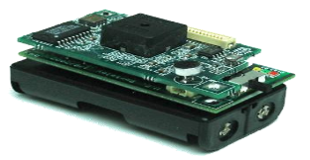
\includegraphics[width=7cm,height=3.7cm]{Chap1/1.png}
	\caption{Différence entre un optimum global et des optima locaux}
	\label{fig:CSF}
\end{figure}

\begin{algorithm}[H]
\caption{Recherche Taboue}
\SetAlgoLined
\DontPrintSemicolon
$ l \gets longueur maximale de la liste taboue $  \;
$ n \gets number of tweaks desired to sample the gradient$ \;
$ S \gets solution initial $ \;
$ Best \gets S $ \;
$ L \gets \{\} $ \;
Insérer s dans L \;

\While{(Best est la meilleure) $\cap$ (nombre iter=max)}{
  \If{ $ longueur(L) > l $ }{
    Défiler un élément de la liste L \;
   }
   $r \gets r’$ où  $r’ \in N(s)$  \;  
   \For{$i\gets1$ \KwTo $N-1$ }{
     $w \gets w’$ où  $w’ \in N(s)$  \;
     \If{$ w \notin L  \cap ( f(w)<f(r) \cup r \in L ) $ }{
		$ e \gets w $ \;
		\If{$ r \notin L  \cap f(r)<f(s) $}{
           $ s \gets r $ \;
           Enfiler r dans L \;
		}
		\If{$f(s)<f(Best)$}{
			$ Best \gets s $			
		}
     }
   }
 }

\end{algorithm}
	
	\item \textbf{Recherche locale : } Pour cette méthode de recherche il suffit de tester itérativement de nouvelles solutions potentielles dans la région de la solution courante, et de prendre la meilleure dans le voisinage. La méthode est une généralisation de la méthode de la descente de gradient elle consiste à partir d’une solution s à choisir une solution s’ dans un voisinage de s, noté N(s). La nouvelle solution choisie est meilleure que la précédente sous la fonction objective. Cela nous permet d’explorer l’espace des combinaisons  de proche en proche, en partant d’une combinaison initiale et en sélectionnant à chaque itération une combinaison voisine de la combinaison courante, obtenue en lui appliquant une transformation élémentaire jusqu’à la convergence à un optimum local. L’algorithme  décrivant le principe général de la recherche locale:

\begin{algorithm}[H]
\caption{Recherche Local}
\SetAlgoLined
\DontPrintSemicolon

$ s \gets solution initial $ \;
\While{ (Best est la meilleure) $\cap$ (nombre iter=max) }{
	$ r \gets s’$ où $s’ \in N(s)$ \;
	\If{ $f(r) < f(s)$ }{
		$ s \gets r $  \;		
	}
}

\end{algorithm}
	
	
	\item \textbf{Recherche à voisinages variables(VNS):} La recherche à voisinage variable (VNS : Variable neighborhood search) est une méta-heuristique proposée par Hansen et Mladenovic en 1997 [28,29]. Elle est basée sur le principe de changement systématique de voisinage durant la recherche (la performance des méthodes de descente).  La procédure de VNS se compose de trois étapes : perturbation (shaking), recherche locale et déplacement. Cet algorithme est efficace si les structures de voisinage sont complémentaires en ce sens qu’un minimum local pour un voisinage n’en n’est pas nécessairement un pour un autre, ce qui veut dire simplement d’utiliser plusieurs voisinages successifs quand on se trouve bloqué dans un minimum local.
	
\begin{algorithm}[H]
\caption{Recherche à voisinages variables (VNS)}
\SetAlgoLined
\DontPrintSemicolon

$ s \gets solution initial $ \;
\Repeat{$ K = K_{Max} $}{
	générer $s’$ ,tel que $s’ \in N(s)$ \;
	$s'' \gets Appel$(Recherche Locale) \;
	\eIf{$f(s'') < f(s)$}{
		$ s \gets s'' $ \;
		$ K \gets 1 $ \;		
	}{
		$ K = K + 1 $ \;
	}
}
	

\end{algorithm}

	
\end{enumerate}



\subsubsection{Méthodes évolutives (A population):}
Depuis le début des années 90, une autre famille d’ heuristiques est devenue très populaire : les Méthodes Évolutives \cite{hertz2000framework} , s’inspirant de la théorie de l’évolution «darwinienne»  tels que le croisement, la mutation et la sélection pour résoudre des problèmes divers. Contrairement à la Recherche Locale qui tente d’ améliorer itérativement une solution courante. Les Méthodes Évolutives travaillent sur une population de solutions en appliquant un processus cyclique composé d’ une phase de coopération et d’ une phase d’adaptation individuelle qui se succèdent à tour de rôle. Dans la phase de coopération, les solutions de la population courante sont comparées entre elles, puis combinées, dans le but de produire de nouvelles solutions qui héritent des bons aspects de chaque membre de la population. Dans la phase d’adaptation individuelle, chaque solution dans la population peut évoluer de manière indépendante. On peut utiliser le même type de critère d’ arrêt que dans la Recherche Locale, ou alors on peut décider de stopper une Méthode Évolutive dès que les solutions dans la population sont jugées trop similaires. Une description générale des Méthodes Évolutives est donnée ci-dessous:

\begin{figure}[h]
	\centering
	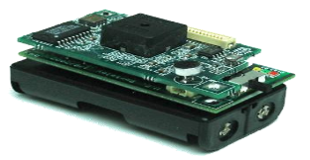
\includegraphics[width=7cm,height=3.7cm]{Chap1/1.png}
	\caption{Principe d’un algorithme évolutionnaire (EA) \cite{dreo2003metaheuristiques}.}
	\label{fig:CSF}
\end{figure}

Le terme Evolutionary Computation englobe une classe assez large de méta-heuristiques qui ont été développés au début des années soixante, telles que les algorithmes génétiques \cite{holland1975adaptation}, les stratégies d’évolution \cite{rechenberg1973evolutionsstrategie} , la programmation évolutive \cite{fogel1966artificial}, et la programmation génétique \cite{koza1992genetic}

\begin{enumerate}[label=\alph*)]
	\item \textbf{Algorithmes génétiques(AG):} développées par J. Holland en 1975 comme outils de modélisation de l’adaptation et qui travaillent dans un espace de chaînes de bits. Elles ont été largement utilisé et développé par D.E. Goldberg en 1989. Cette classe s’inspire de la théorie de l’évolution et des règles de la génétique qui expliquent la capacité des espèces de s’adapter à leurs environnement à l’ aide de l’ opérateur de mutation, alors que l’ échange               	d’information est gouverné par un opérateur de reproduction et un opérateur de combinaison (ou croisement). L’algorithme ci-dessous décrit ce principe général, dont les principales étapes sont détaillées ci-après.

\begin{algorithm}[H]
\caption{Algorithme génétique}
\KwResult{la meilleure combinaison ayant appartenu à la population }
\SetAlgoLined
\DontPrintSemicolon

Initialiser la population avec un ensemble de combinaisons de E \;
\While{critères d’arrêt non atteints}{
	Sélectionner des combinaisons de la population \;
	Créer de nouvelles combinaisons par croisement et mutation \;
	Mettre à jour la population  \;
}

\end{algorithm}


\begin{figure}[h]
	\centering
	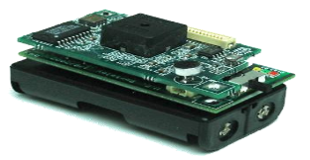
\includegraphics[width=7cm,height=3.7cm]{Chap1/1.png}
	\caption{Principe d’un algorithme évolutionnaire (EA) \cite{dreo2003metaheuristiques}.}
	\label{fig:CSF}
\end{figure}
	
\begin{itemize}
	\item \textbf{Initialisation de la population: }en général, la population initiale est générée de façon aléatoire, selon une distribution uniforme assurant une bonne diversité des combinaisons. Une solution initiale est de bonne qualité, celle qui nous permet de converger vers un optimum global dans le plus court délai possible.
	
Il est à noter que cette méthode est utilisée dans toutes les méta-heuristiques avec population.

	\item \textbf{Sélection: } cette étape consiste à choisir les combinaisons de la population qui seront ensuite croisées et mutées. Il s’agit là de favoriser la sélection des meilleures combinaisons, tout en laissant une petite chance aux moins bonnes combinaisons. Il existe de nombreuses façons de procéder à cette étape de sélection. Par exemple, la sélection par tournoi consiste à choisir aléatoirement deux combinaisons et à sélectionner la meilleure des deux (ou bien à sélectionner une des deux selon une probabilité dépendant de la fonction objectif).
	
	\item \textbf{Croisement:} est une opération de diversification. cette opération consiste à générer de nouvelles combinaisons, à partir des deux individus sélectionnés. Là encore, il existe de nombreux opérateurs de croisement. Une méthode simple consiste à choisir aléatoirement un point de croisement, à couper chaque combinaison parente en ce point, puis à reformer deux enfants en échangeant les parties composant les parents de part et d’autre du point de croisement.
	
	\item \textbf{Mutation: } cette opération consiste à modifier de façon aléatoire certains composants des combinaisons obtenues par croisement.
	
	\item \textbf{Mise à jour de la population: } cette étape consiste à remplacer certaines combinaisons de la génération précédente par certaines combinaisons issues des opérations de croisement et de mutation, formant de la sorte une nouvelle génération. Là encore, il existe différentes stratégies de remplacement, favorisant plus ou moins la diversité, et plus ou moins élitistes. On peut par exemple choisir de ne garder que les meilleurs individus, qu’ils soient issus de la nouvelle génération ou de l’ancienne, ou bien ne garder que les individus de la nouvelle génération, indépendamment de leur qualité.
	
	\item \textbf{Critères d’arrêt: } le processus d’évolution est itéré, de génération en génération, jusqu’à ce qu’une combinaison de qualité suffisante soit générée, ou bien jusqu’à ce qu’une limite de temps soit atteinte. On peut également utiliser des indicateurs de diversité (comme par exemple le taux de ré-échantillonnage ou la distance pair-à-pair) pour arrêter le processus lorsque la population est devenue trop uniforme. On peut aussi limiter le nombre d’itération possible ou encore les probabilités d’application des opérateurs de croisement et de 
mutation.
 
\end{itemize}	

	
	\item \textbf{L’optimisation des colonies de fourmis (ACO): }est une technique d’intelligence artificielle qui s'inspire du comportement intelligent des fourmis lors de la recherche de nourriture. Cette méta-heuristique permet de trouver des solutions de haute qualité aux problèmes d’optimisation combinatoire. 

En raison de leur comportement de recherche de nourriture, les fourmis trouvent les chemins les plus courts entre leur nid et leur source de nourriture, en déposant sur la terre une substance chimique appelée phéromone. Cela forme une traînée de phéromone qui est utilisée pour la communication stigmergique. La présence d'une telle phéromone sur les trajectoires affecte la prise de décision des fourmis concernant les trajectoires choisies par elles. Les fourmis sélectionnent de manière probabiliste les chemins marqués par de fortes concentrations de phéromones ce qui permet aux fourmis de trouver le chemin le plus court vers la source de nourriture.

\begin{algorithm}[H]
\caption{L’optimisation des colonies de fourmis (ACO)}
\KwResult{la meilleure solution trouvée}
\SetAlgoLined
\DontPrintSemicolon

Initialisation : initialisation de phéromones et les paramètre avec des valeurs constantes \;
Construction de la solution initiale \;
\While{condition d’arrêt non atteinte }{
	\While{nombre de fourmis non atteint}{
		Construction d’une solution selon la concentration de phéromone \;
		Mise à jour en ligne de  la table des phéromones \;
	}
	\If{la meilleure solution trouvée par l’itération courante est meilleure que celles des 	itérations précédente}{
		Mise à jour de l a solution courante \;
	}
	Mise à jour hors ligne de  la table des phéromones \;	
}

\end{algorithm}

\begin{itemize}
	\item \textbf{Solution initiale:} en général, la solution initiale est générée de façon aléatoire.Une solution est composée de plusieurs attributs définis selon la nature du problème.
	
	\item \textbf{Initialisation de la table de phéromone:} la table de phéromone contient  la concentration de phéromone pour tous les attributs possible d’une solution. Au départ tous les attributs ont une même concentration de phéromone. 
	
	\item \textbf{Mise à jour de phéromone:}
		\begin{itemize}
			\item \textbf{En ligne:} les attributs communs entre la solution courante et la meilleure solution vont être favoriser par une valeur constante supplémentaire.
			\item \textbf{Hors ligne:} les attributs appartenant à la meilleure solution vont être favoriser par la valeur constante. 
		\end{itemize}
\end{itemize}
	
	\item \textbf{L’algorithme à base de biogéographie (BBO)} BBO est un algorithme inspiré de la biogéographie, qui étudie la répartition géographique des organismes biologiques. 

Tout comme GA et PSO qui sont basés sur la biologie, BBO est un algorithme basé sur une population dans lequel chaque population de solutions candidates est utilisée dans la procédure de recherche d’un optima global. BBO présente certaines caractéristiques communes avec l’algorithme d'optimisation, le GA. En GA, un individu de la population s'appelle un chromosome et a sa propre valeur de condition physique. De même, dans BBO, chaque individu est qualifié d'habitat et a son indice de qualité de l'habitat (HSI) pour évaluer sa qualité en tant que solution. Comme nous avons affaire à un problème de minimisation, un habitat à faible indice de sécurité d'impact représente une bonne solution et un habitat à haut indice de faiblesse est plutôt une solution médiocre. Chaque chromosome de GA est constitué de gènes, tandis que, pour BBO, chaque habitat est caractérisé par des variables d'indice de pertinence (SIV). L'AG compte deux opérateurs principaux: le croisement et la mutation. Pendant ce temps, chez BBO, les principaux opérateurs sont la migration et la mutation. L'opérateur de migration est composé d'émigration et d'immigration. Il est utilisé pour améliorer et faire évoluer les habitats (solutions au problème d'optimisation) de la population. Les fonctionnalités de solution (SIV) émigrent d'habitats à faible HSI (habitats d'émigration) vers des habitats à haut HSI (habitats d'immigration). Il existe différentes alternatives pour les processus de migration et de mutation de BBO. La manière dont nous implémentons ces deux opérateurs est expliquée en détail dans le prochain chapitre. 

\begin{algorithm}[H]
\caption{L’algorithme à base de biogéographie (BBO)}
\KwResult{la meilleure solution ayant appartenu à la population }
\SetAlgoLined
\DontPrintSemicolon

Générer aléatoirement un ensemble de solutions initiales (îles) \;
\While{le critère d’arrêt n’est pas atteint}{
	Évaluer la fitness (HSI) de chaque solution \;
	Calculer le nombre d’espèce S, le taux d’immigration $\lambda$ et d’émigration $\mu$ pour chaque solution \;
	Migration  \;
	Mutation : muter les individus au taux de mutation \;
	Remplacement de la population par les descendants \;
	Implémenter l’élitisme \;
}

\end{algorithm}
	
	\item \textbf{Algorithmes mémétiques (algorithme de colonies de fourmis \& d’essaim de particules) : }
Le terme «algorithmes mémétiques»  est apparu pour la première fois dans [38], introduit par Moscato en 1986. L’idée principale de ce genre d’algorithme est de rendre plus agressif un algorithme génétique par l’ajout d’une recherche locale en plus de la mutation.

La faible vitesse de convergence est la première observation provenant de l’implémentation de l’algorithme génétique. Pour cet effet Moscoto a pensé d’ajouter une recherche locale  qui peut être une méthode de descente ou une recherche locale plus évoluée (recuit simulé ou recherche tabou par exemple). Cette recherche locale sera appliquée à tout nouvel individu obtenu au cours de la recherche.

D’une vue globale, l’application de cette simple modification n’influe en rien sur le comportement de l’algorithme, mais  cela peut apporter de profondes changement en ce dernier. Après avoir créé un nouvel individu à partir de deux parents sélectionnés, on applique une recherche locale et sous certaines conditions on applique un opérateur de mutation à cet individu. Les conditions peuvent être une certaine probabilité. Il est aussi possible d’ajouter un critère d’aspiration ou d’autres techniques plus évoluées à cet endroit.\\


\begin{algorithm}[H]
\caption{Simple Algorithme mémétique}
\KwResult{la meilleure solution ayant appartenu à la population }
\SetAlgoLined
\DontPrintSemicolon

Initialisation : générer une population initiale $P$ de solutions de taille $| P | = n$  \;
\Repeat{critère d'arrêt satisfait}{
	Sélection: choisissez 2 solutions s et $s’$ avec la technique volue \;
	Croisement: combinez les solutions parentes s et $s’$ pour former une solution enfant $y$ \;
	Recherche locale: appliquer une procédure de recherche locale sur y sous certaines conditions \;
	Mutation: appliquer un opérateur de mutation sur y dans des conditions \;
	Choisir un individu y’ à remplacer dans la population \;
	remplacer y’ par y dans la population \;	
}

\end{algorithm}

\paragraph{•}

\begin{figure}[h]
	\centering
	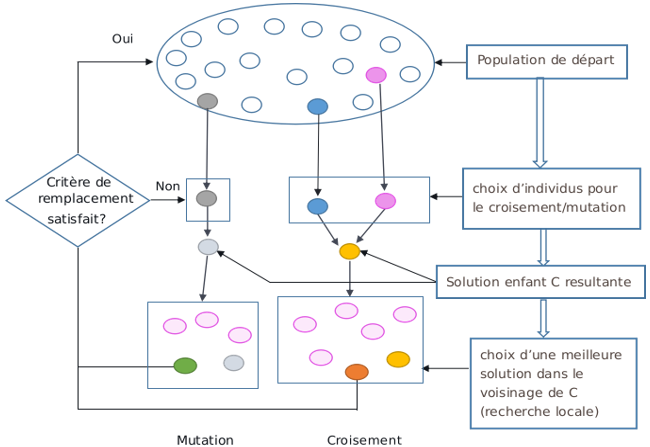
\includegraphics[width=15cm,height=9cm]{Chap3/7.png}
	\caption{Schéma explicatif d’un algorithme mémétique}
	\label{fig:CSF}
\end{figure}
	
\end{enumerate}


\section{Conclusion}
Nous avons présenté dans ce chapitre l’état de l’art des méta-heuristiques pour l’optimisation des problèmes Np-difficile. Plus de détails sur le problème de l’arbre dominant qui en est un, ainsi que les méthodes utilisées pour sa résolution seront mis au clair dans le prochain chapitre.



\cleardoublepage

\addcontentsline{toc}{chapter}{\numberline{}4eme chapiter}
\addtocontents{lof}{\textbf{Chapter A4}}

\setcounter{chapter}{4}
\setcounter{section}{0}
\setcounter{figure}{0}
%\setcounter{algorithm}{0}

\begin{center}
	\Huge\textbf{4eme chapter}
\end{center}

\section{Introduction}
Dans les chapitres précédents, nous avons introduit différentes techniques utilisées pour la résolution des problèmes d’optimisation combinatoire, notamment les méthodes adoptées pour la résolution du problème de l’arbre dominant DTP, dont une grande majorité a servi de source d’inspiration pour l’élaboration des approches que nous avons proposé et qui seront détaillées le long de ce chapitre.  Nous allons dans un premier présenter les structures de données utilisées pour représenter les données du problème ainsi que la solution.

\section{Représentation du graphe modélisant le problème}
Un WSN est un graphe pondéré non orienté $G=(V,E,w)$, où $V$ est l’ensemble des nœuds du réseau, E l’ensemble des arêtes et w un poids non négatif attribué pour chaque arête $e=(u,v)$. 

Nous utilisons pour représenter le WSN deux vecteurs, un vecteur de taille $|V|$ contenant des entiers représentant chaque nœud et l’autre est de taille $|V-1|$ il contient une structure d’arc (nœud 1, nœud 2 et le poids entre les deux nœuds. Nous allons dans ce qui suit présenter le codage de la solution ainsi que la méthode d'extraction du DT à partir de cette solution.


\section{présentation d’une solution:}
Nous proposons de représenter une solution en utilisant le codage binaire qui est considéré dans la littérature comme un bon moyen pour manipuler les différents gène (position(bit) dans une solution) d’une solution pour une population donnée. Si le gène est égale à '1', cela veut dire que le nœud correspondant est actif, s'il vaut '0', il est inactif.


\section{Méthode d'extraction d'un arbre dominant à partir du vecteur solution:}
Au départ nous avons deux vecteurs $(Vect, DN)$, où, $Vect$ contient tous les nœuds de notre graphe, $DN$ est un vecteur binaire de taille $|V|$ initialement null et contiendra par la suite l’ensemble des nœuds dominant .

L’ajout des nœuds à $DN$ se fait via un processus itératif. A chaque fois un nœud est choisi d’une façon aléatoire,  et est ajouté à $DN$. Ce processus poursuit son fonctionnement tant que les nœuds appartenant à $DN$ ne couvre pas tous le graphe ou ils ne sont pas  connectés. On dit que $DN$ couvre le graphe si et seulement si tous les nœuds de notre graphe sont soit dans $DN$ soit adjacent à un autre nœud qui est dans $DN$.

Pour pouvoir construire un DT, il faut d’abord vérifier  que les nœuds actifs dans $DN$  sont connectés entre eux. Dans le meilleur des cas, les nœuds actifs dans $DN$ sont connectés ; Dans le cas contraire nous devons les rendre connecté en utilisant une méthode de connection décrite si après.

\section{La méthode de connection:}
Soit un vecteur DNC initialement vide qui va contenir par la suite ensemble de nœuds connecté. En premier lieu, nous retirons un nœud aléatoirement de DN et nous l’insérons dans DNC. Puis, d’une façon itérative, nous retirons tous les nœuds de DN qui ont au moins un voisin dans DNC et nous l’insérons dans DNV. En second lieu nous, devons insérer tous les nœuds actifs dans DN dans DNC en utilisant une autre fonction. Cette fonction consiste au départ, à choisir un nœud v aléatoirement dans V qui n’est pas dans DNC. Si v a au moins deux voisins un dans DN et l’autre dans DNC, alors nous retirons son voisins dans DN et nous l’insérons  avec v dans DNC. Si aucun nœud n’est trouvé nous procédons à une sélection par pair de nœuds où chaque nœud entre eux a soit un voisin dans DN ou dans DNC et nous refaisions le même processus de recherche daans le cas d’un seul nœud à selectionner. Nous ré-exécutons ce prceossus jusqu'à DN devient null.

Une fois que l’ensemble DN soit null, nous appliquant la méthode d’élagage et MST décrit dans le chapitre 3. Nous aurons au final, un arbre dominant DT, représenté sous forme d’un vecteur de type arc (chaque élément de ce vecteur est composé d’un noeud1, noeud2, et le poids entre ces deux nœuds).


\section{Approche proposée:}
Dans ce mémoire nous avons proposé plusieurs approches pour résoudre le DTP. Nous avons proposé de le résoudre dans un premier temps en utilisant des méta-heuristiques, et en utilisant la coopération de ces méta-heuristiques dans un second temps. Nous allons structurer ce qui suit en deux parties. Dans la première partie, nous présentons chacune des méta-heuristiques utilisées, dans la seconde partie, nous présentons l'approche coopérative.


\subsection{description des méta-heuristiques utilisées}
La méthode de résolution du problème de l’arbre dominant que nous avons proposée consiste à intégrer un processus de recherche locale  à la méta-heuristiques. Nous allons dans ce qui suit décrire les approches proposées. 

\subsubsection{Ant colony optimisation}
Nous utilisons dans cette première solution, l'algorithme des colonies de Fourmies pour résoudre le DTP. Nous allons décrire dans ce qui suit l'adaptation des operateurs de  cette métaheuristique au problème étudié. 

\begin{enumerate}
	\item \textbf{Les opérateurs de l’algorithme ACO}\\
\begin{enumerate}[label=\alph*)]
	\item \textbf{Recherche locale:}\\
	Dans la recherche locale que nous proposons, supposons que nous avons une solution. Nous parcourons le vecteur de la solution et on inverse la valeur des élément (si la valeur d’un élément est égale à 1, elle devient 0 ou inversement) . A chaque fois que nous inversons  la valeur  de chaque élément nous faisons une évaluation de la fonction objectif. A tous coups où la solution est améliorée, cette dernière est sauvegardé et la recherche d’une meilleure solution se fera à partir de cette solution.
	
La recherche se terminera lorsque touts  les nœuds dominants aurons été parcourus.
il est à noter que la méthode de recherche locale citée ci dessus est utilisée dans toutes les solutions proposées.
	
	\item \textbf{Les méthodes de sélection:}\\
	Nous proposons d'utiliser deux méthodes de sélection d’individus. Ces deux méthodes ont été retenues après une série d'expérimentations faisant apparaître les deux méthodes donnant les meilleurs résultats.

	\begin{itemize}
		\item \textbf{Méthode de sélection par Intensification: }\\
		Son principe consiste à choisir le nœud ayant la plus grande probabilité pour améliorer la solution 
		
		\item \textbf{La sélection par tournoi}\\
		le principe de cette sélection consiste à choisir deux nœuds aléatoirement, puis de retenir celui ayant la meilleure probabilité 
	\end{itemize}
\end{enumerate}
	


	\item \textbf{Fonctionnement de l’algorithme ACO}\\
L’algorithme de colonie de fourmi est une approche métaheuristique basée sur une  population et inspirée du comportement des fourmis réelles. L’idée principale derrière cette méthode provient de l’observation de la capacité des fourmis pour trouver le plus court chemin entre une  source de nourriture et le nid.
Cette méta-heuristique est composée d’une phase d’initialisation et d’une phase itérative. La première phase consiste à initialiser une solution de départ qui sera décrite ci-dessous. Elle comprend également l’initialisation du vecteur des probabilités et de la table de phéromone.

Ensuite, pour chaque itération, chaque fourmi construit sa solution en choisissant aléatoirement une méthode de sélection (intensification - sélection par tournois). Après avoir construit une solution la recherche locale est lancée pour atteindre un résultat meilleure. La meilleure solution retournée par la fourmi courante va participer à la mise à jour du vecteur de probabilité( mise à jour en ligne ) en appliquant la formule (1). A la fin de chaque itération, la meilleure solution trouvée par la population de fourmis va elle aussi participer à la mise à jour du vecteur de probabilité  (mise à jour hors ligne) avec la formule suivante:

\begin{equation}
	\mathlarger{
		p_{ij}^k = \frac{
				[T_j]^\alpha \, [n_{ij}]^\beta
			}{
				\mathlarger{\sum}_{h \in S} \, \mathlarger{\sum}_{l \in N_h^k} \, [T_l]^\alpha \, [n_{hl}]^\beta
			}
	}
\end{equation}


où:\\
$T_j$ la concentration de phéromone du nœud $j$ \\
$n_{ij}$ est le terme heuristique qui vaut $1 / w_{ij}$, dont $w_{ij}$ est le poids de l’arc du nœud $i$ vers le nœud $j$.\\
$\alpha \, , \beta$ sont deux paramètres qui déterminent l'influence relative de la trace de phéromone et de l'information heuristique dans le processus de génération des solutions. \\
$N_h^k$ est l'ensemble de sommets non sélectionnés adjacents à un sommet $h \in S$. \\

Nous allons décrire dans ce qui suit, l'approche de construction de la solution initiale. Soit S l'ensemble des solutions (initialement vide). Tous les sommets de notre graphe sont étiquetés initialement comme non marqués. Un sommet v est sélectionné aléatoirement dans l'ensemble V puis  ajouté à S. Ce sommet est étiqueté comme marqué et tous les sommets adjacents à ce sommet deviennent marqués. Après cela, à chaque étape, la fourmi k construit une solution en sélectionnant un sommet non sélectionné v adjacent à un sommet déjà sélectionné $u \in S$. La sélection de ce sommet non sélectionné v est déterminée de manière probabiliste.


Après que tous les sommets du graphe soient étiquetés à marqué. Les fonction élagage et MST décrit dans le chapitre 3 sont appliquées.\\

Le pseudo-code de ACO est donné dans l’algorithme 1 suivant:

\begin{algorithm}[H]
\caption{ACO DT}
\KwData{Un graphe général pondéré non orienté $G = (V, E, w) $}
\KwResult{Un DT  optimal de G }
\SetAlgoLined
\DontPrintSemicolon

Initialiser le vecteur de probabilité ainsi que la table de pheromone \;
Construction de la solution initiale \;

\While{le nombre d’itération non atteint }{
	\For{chaque fourmi}{
		Construction d’une solution \;
		Recherche locale() \;
		Mise à jour de la table de phéromone. Selon la meilleure solution trouvée par la fourmi \;
	}
	Mise à jour de la table de phéromone Selon la meilleur solution atteinte par les fourmis\;	
}
	
\end{algorithm}
	
\end{enumerate}



\subsubsection{Algorithme génétique}
Nous allons décrire dans ce qui suit les opérateurs retenus dans l'approche utilisant les algorithmes génétiques. 


\begin{enumerate}
	\item \textbf{Les opérateurs de l’algorithme ACO}\\

\begin{enumerate}[label=\alph*)]
	\item \textbf{Génération de la Population initiale:}\\
	La population initiale est construite avec un ensemble de solutions (individu) définies aléatoirement. La taille de chaque individu est le même nombre de nœuds dans un réseaux de capteurs sans fil.


	\item \textbf{Codage des éléments d’une population: }\\
	Le codage utilisé dans cette approche est celui décrit dans la section II.
	
	\item \textbf{La méthode de croisement utilisée:}\\
	Pour cet algorithme nous avons utilisé la méthode de croisement uniforme. Il opère à l’aide d’un masque construit aléatoirement, pour décider lequel des parents va transmettre  la valeur du gène à l’un ou l’autre des descendants. Si à la même position que le gène, la valeur du masque est égale à 1, le gène du parent 1 passe à celui de l’enfant 1 et le gène du parent 2 passe à l’enfant 2. Sinon, c’est l’inverse qui se produit (figure \ref{fig:ECU}). Cette fonction renvoie l’enfant ayant la meilleur qualité (le poids minimal).\\
La figure \ref{fig:ECU} illustre se processus par un exemple.

\begin{figure}[H]
	\centering
	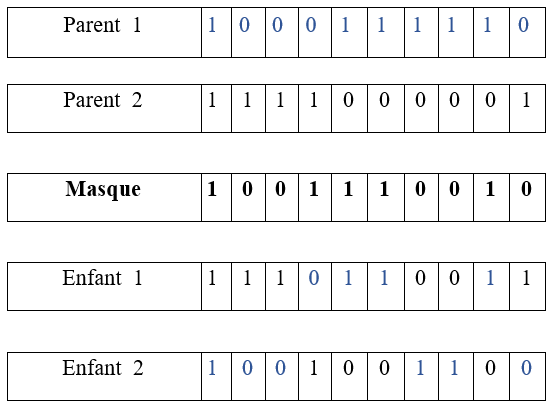
\includegraphics[width=12cm,height=6.5cm]{Chap4/1.png}
	\caption{Exemple de croisement uniforme}
	\label{fig:ECU}
\end{figure}
	

	\item \textbf{Mutation:}\\
	La mutation est une autre solution pour créer de nouveaux individus  et de modifier ceux déjà existant. Le hasard dans cette méthode va nous être d’une grande utilité. Dans notre cas, un index généré aléatoirement va décider dans quelle position le gène à muter se trouve. Rien ne nous dit que l’individu muté sera meilleure ou au moins bon, mais il pourrait être efficace pour la création de  bonnes solutions.  Un exemple illustratif sera représenté par  la figure 4.2.

\begin{figure}[H]
	\centering
	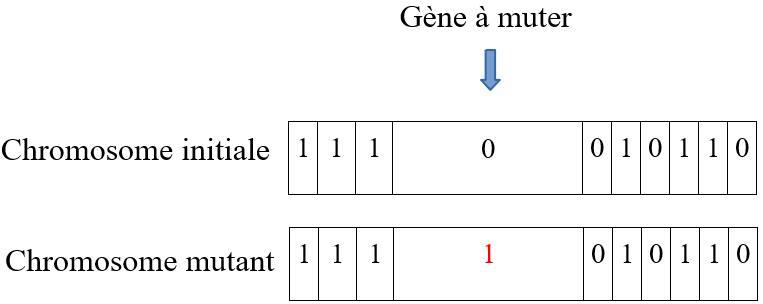
\includegraphics[width=13cm,height=4cm]{Chap4/2.png}
	\caption{Représentation schématique de la mutation}
	\label{fig:RSM}
\end{figure}


	\item \textbf{Élitisme:}\\
Cet opérateurs permet de garder les meilleurs individus de chaque population. Notre méthode d’élitisme consiste à remplacer les m mauvais individus de la nouvelle population par les m meilleurs individus de la  population précédente. 

\end{enumerate}


\item \textbf{Fonctionnement de l’algorithme génétique (GA)}

Après avoir créé une population initiale, l’algorithme GA procède comme suit:

\begin{algorithm}[H]
\caption{Génétique DT}
\SetAlgoLined
\DontPrintSemicolon

Initialiser une population d’une façon aléatoire \;

\While{$ i < $ Nombre d’itération}{
	\While{$j<PopSize$}{
		Récupérer deux individu de la population $n_1 , n_2$ \;
		$Enfant = Croisement(n_1,n_2)$ \;
		rand = Générer une valeur aléatoire entre 0 et 100\;
		\If{rand < 5\% }{
			Mutation(Enfant)\;		
		}
		Recherche locale() \;
		Ajouter le meilleur individu à la nouvelle population \;
	}
	Elitisme() \;
}

\end{algorithm}


\end{enumerate}


\subsubsection{biogeography based optimimisation (BBO)}
C’est une méta heuristique qui fait partie des algorithmes évolutionnaire basée sur la biogéographie. Dans ce qui suit, nous allons présenter l’approche BBO développée pour la résolution du problème de l’arbre dominant ainsi que ses opérateurs.

\begin{enumerate}
	\item \textbf{Les opérateurs de l’algorithme BBO}\\
	\begin{enumerate}[label=\alph*)]
		\item \textbf{Génération de la Population initiale:}\\
	\end{enumerate}	
	
	\item \textbf{Le fonctionnement de l’algorithme BBO}\\
	
	
\end{enumerate}



\subsection{Description de l'approche coopérative}
Nous proposons une approche  coopérative entre les méta-heuristiques pour la résolution du problème de l’arbre dominant où une méta-heuristique maître contrôle plusieurs méta-heuristiques esclaves. Les points forts d'une méta-heuristique esclave compensent les points faibles d'une autre grâce à la notion de rang. Le rang est un moyen de mettre en valeur les points forts des méta-heuristiques esclaves. Il est attribué par le maître et est égale à 0 au départ. Il est mis à jour continûment par la méta-heuristique maître qui augmente le rang des méta-heuristiques esclaves ayant amélioré la solution et diminue le rang de celles qui ne l'auront pas amélioré. Cette mise à jour tend à récompenser les méta-heuristiques esclaves qui auront réussi à améliorer la solution courante. Comme conséquence, les méta-heuristiques esclaves ayant un rang élevé participeront donc davantage au développement de la solution finale.




\MemChapter{Étude expérimentale}

\addtocontents{lof}{\textbf{Étude expérimentale}}

\section{Introduction}
Dans le chapitre précédent, nous avons présenté en détail les approches que nous avons proposées pour la résolution du problème de l’arbre dominant (DTP). Nous allons présenter dans ce qui suit une étude expérimentale effectuée pour comparer les résultats des approches proposées avec d’autres approches développées pour la résolution du DTP. Nous clôturons avec une conclusion.


\section{Environnement de travail}

\subsection{Environnement matériel}
Pour les tests effectués nous avons utilisé une machine. Les caractéristiques de  machine sont données dans la figure \ref{fig:CMU}.

\begin{figure}[H]
	\centering
	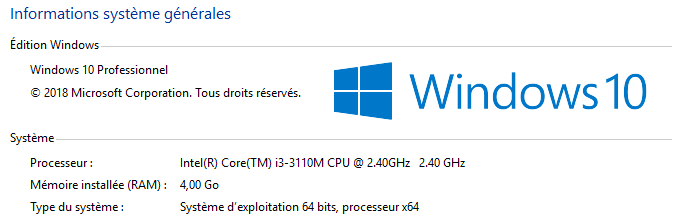
\includegraphics[width=16cm,height=7cm]{Chap5/1.png}
	\caption{Caractéristiques de la machine utilisée}
	\label{fig:CMU}
\end{figure}

\subsection{Environnement logiciel}
Nous avons opté pour le langage Java pour la programmation, car il offre une grande flexibilité et facilite l’implémentation qui est due au fait qu’il soit totalement orienté-objet.

\textbf{IDE :}
L’environnement de développement choisit est IntelliJ IDEA, spécialement dédié au développement en utilisant le langage Java. Il est proposé par l’entreprise JetBrains et est caractérisé par sa forte simplicité d’utilisation et les nombreux plugins et extensions qui lui sont dédiées.

\section{Jeux de données utilisées}
Afin de tester l'approche proposée, nous avons opté pour l'utilisation de fichiers benchmark qui vont représenter des instances du problème. Les différentes instances sur lesquelles notre étude s'est portée sont dérivées à partir des mêmes benchmarks de \cite{sundar2013new}. Une instance est considérée comme un graphe de disques, G = ( V, E ) où chaque disque représente la plage de transmission de chaque nœud. Le poids de chaque arête $e_{uv} \in E $ est défini sous la forme w ( u, v ) = $d_{uv}^2$, où $d_{uv}$  est la distance euclidienne entre deux nœuds u et v. L'hypothèse est que tous les nœuds sont répartis de manière aléatoire dans une zone de $500m * 500m $  et la plage de transmission de chaque nœud est de 100 m.


\section{Expérimentation}
Pour montrer l'efficacité de l'approches proposées nous ne nous sommes pas limité à des instances de problème ayant un certain nombre de nœuds.

Nous nous avons effectué cela pour une large plage de nombre de nœuds (50 - 500).

Pour ACO, nous avons utilisé une population de 15 fourmis. Nous avons utilisé $\alpha = 1 \, , \, \beta = 1 \, , \, p = 0.05 \, , \, P_0 = 0.1 $. Toutes les valeurs de phéromone initiales sont égales à 0,05. Pour BBO et GA, la taille de la population est de 20 individus. Quant à l’approche de coopération,  nous avons utilisé 0.5 comme probabilité initiale et 0,1 pour la valeur de  \( \alpha \).

Pour toutes les instances du test, nous avons opté pour 100 itérations pour chacune des approches proposées. Nous avons jugé que ce nombre d'itérations est suffisant pour une qualité quasi optimale de la solution. Donner plus d'itérations à nos approches que celles mentionnées ci- dessus n'aura que peu d'impact sur la qualité de la solution. 

Toutes ces valeurs de paramètres sont choisies empiriquement. Ces valeurs de paramètres donnent de bons résultats pour la majorité des instances de test.

\subsection{Étude comparative}
Afin de mener à bien une étude comparative entre nos approches et d’autres travaux effectués pour la résolution du DTP, nous avons gardé approximativement le même nombre d’évaluations de la fonction objectif.

Dans le but d’assurer l’intégrité des résultats, nous avons effectué un total de 20 exécutions pour chacune des instances. Les résultats d’exécutions de nos approches (ACO, BBO, GA et la méthode coopérative) sur les instances citées auparavant, sont illustrés dans le Tableau \ref{tab:1}.

Dans le Tableau  \ref{tab:1}, les lignes correspondent aux différentes instances étudiées, quant aux colonnes, elles représentent, pour chaque approche : la meilleure solution obtenue (colonne BS), la moyenne de toutes les solutions obtenues sur les 20 exécutions (colonne AVG), le nombre d’évaluations nécessaire pour trouver la meilleure solution (colonne NBV) et la colonne qui représente le temps d’exécution de chaque métaheuristique en seconde (colonne sec). 
Notez que les meilleures valeurs sont indiquées en gras dans les tableaux comparatifs.


\begin{table}[H]
	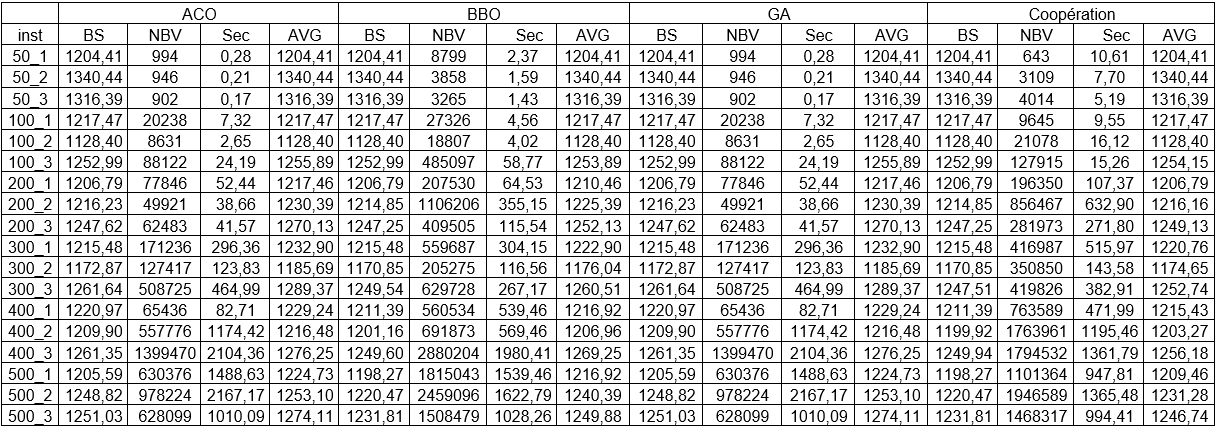
\includegraphics[width=17cm,height=7cm]{Chap5/t1.png}
	\caption{Résultats d’exécutions des  approches proposées}
	\label{tab:1}
\end{table}


\subsubsection{Comparaison de la méthode coopérative avec les autres approches}
Dans ce qui suit nous allons présenter une comparaison entre notre approche coopérative et les autres approches que nous avons développées. Cette comparaison a pour but de montrer l’efficacité de notre approche coopérative par rapport aux approches développées. 

\begin{enumerate}[label=\alph*)]
	\item \textbf{Avec l’approche ACO}\\
	D’après le graphe de la figure \ref{fig:DEMACOMC} et les résultats présentés dans le tableau \ref{tab:2}, les résultats des deux approches sont similaires pour les 11 premières instances. La meilleure solution (BS) obtenue par l’ approche coopérative  est meilleure que celle obtenue par ACO pour les sept  (7) dernières instances. Il faut également noter que la qualité moyenne des solutions (AVG) obtenue par la méthode de coopération est  meilleure que celle d’ACO pour la majorité des instances du problème. Comparé à ACO, le nombre d’évaluation donnée par  l’approche de coopération est relativement faible. Enfin,  le temps d’exécutions  d'ACO en général est moins important.

\begin{table}[H]
	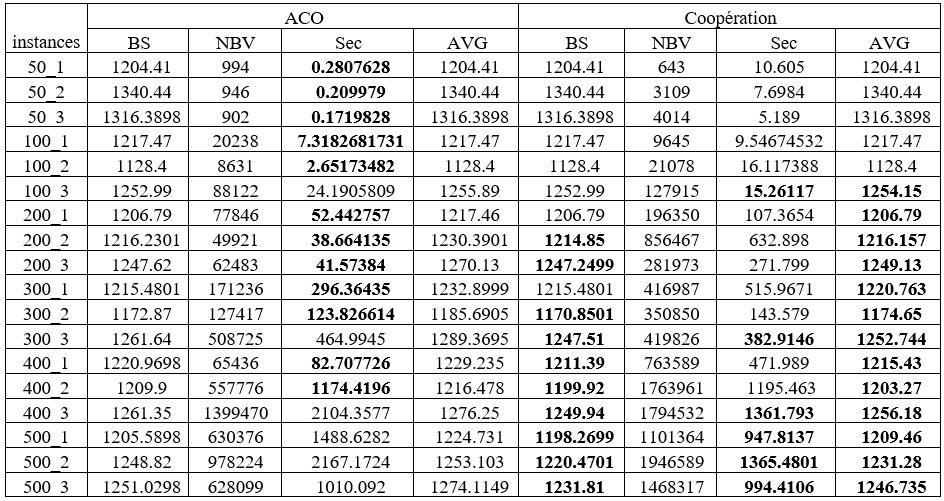
\includegraphics[width=15cm,height=8cm]{Chap5/t2.png}
	\caption{Résultats d’exécutions d’ACO et la méthode de coopération}
	\label{tab:2}
\end{table}

\begin{figure}[H]
	\centering
	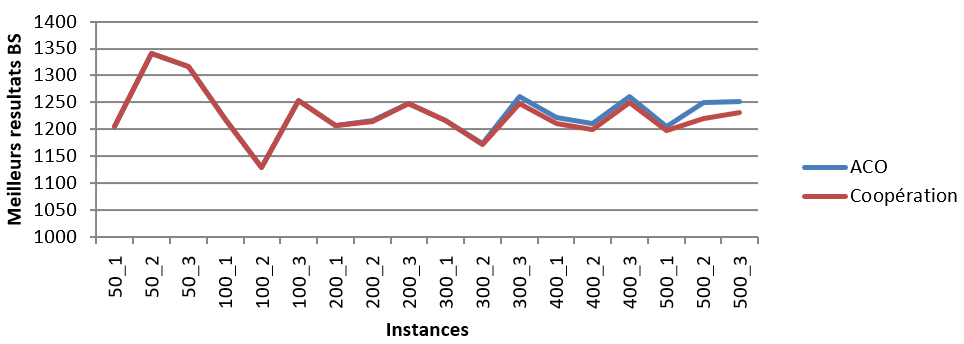
\includegraphics[width=16cm,height=7cm]{Chap5/2.png}
	\caption{Diagrammes d’exécutions de la méthode ACO et la méthode coopérative}
	\label{fig:DEMACOMC}
\end{figure}

	\item \textbf{Avec l’approche BBO}\\
D’après le graphe de la figure \ref{fig:DEMBBOMC} les deux approches sont similaires. De même, en analysant le tableau \ref{tab:3}, la meilleure solution (BS) obtenue par la méthode BBO et celle obtenue par l’approche de coopération est pratiquement la même.

Concernant les moyennes des solutions (AVG), celles obtenues par l’approche coopérative sont de meilleures qualités par rapport à celles obtenues par BBO.

Pour ce qui est du nombre d'évaluations celui de l’approche coopérative est négligeable comparé à l’autre approche.

\begin{table}[H]
	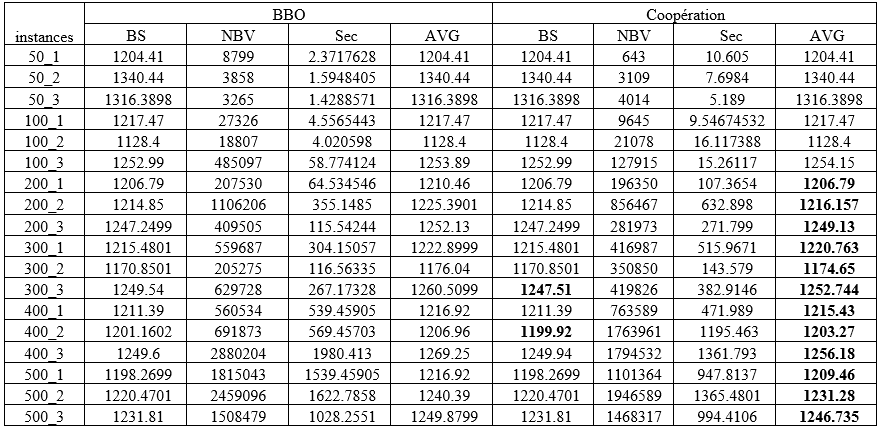
\includegraphics[width=15cm,height=8cm]{Chap5/t3.png}
	\caption{Résultats d’exécutions de BBO et la méthode de coopération}
	\label{tab:3}
\end{table}

\begin{figure}[H]
	\centering
	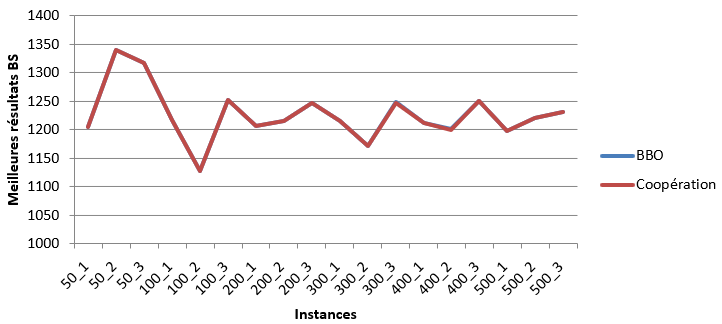
\includegraphics[width=16cm,height=7cm]{Chap5/3.png}
	\caption{Diagrammes d’exécutions de la méthode BBO et la méthode coopérative}
	\label{fig:DEMBBOMC}
\end{figure}

	\item \textbf{Avec l’approche GA}\\	
D’après le graphe de la figure \ref{fig:DEMGAMC} et les résultats présentés dans le tableau \ref{tab:4}, les deux approches sont similaires pour les 11 premiers instances, la meilleure solution (BS) obtenue par l’ approche coopérative  est meilleure que celle obtenue par GA pour les sept  (7) dernieres instances. Il faut également noter que la qualité moyenne des solutions (AVG) obtenue par la méthode de coopération est de meilleure qualité que celle obtenue par GA pour toutes les instances du problème. Comparé à GA, le nombre d’évaluation donnée par  l’approche de coopération est relativement faible.

\begin{table}[H]
	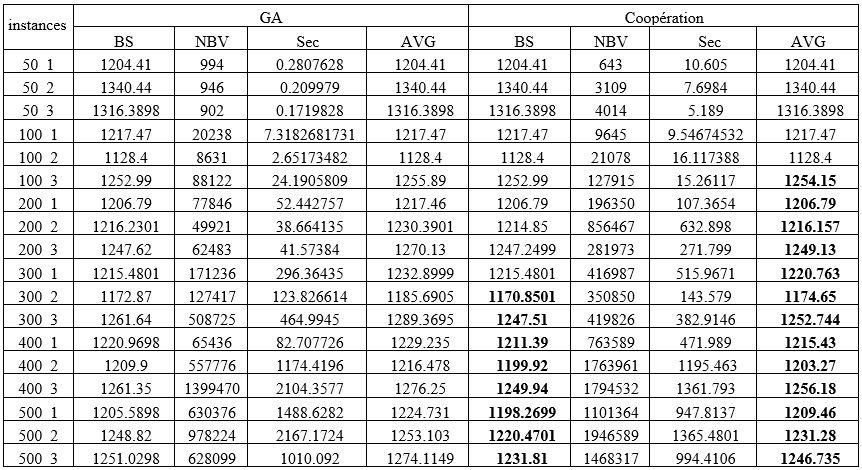
\includegraphics[width=15cm,height=8cm]{Chap5/t4.png}
	\caption{Résultats d’exécutions de GA et la méthode de coopération}
	\label{tab:4}
\end{table}

\begin{figure}[H]
	\centering
	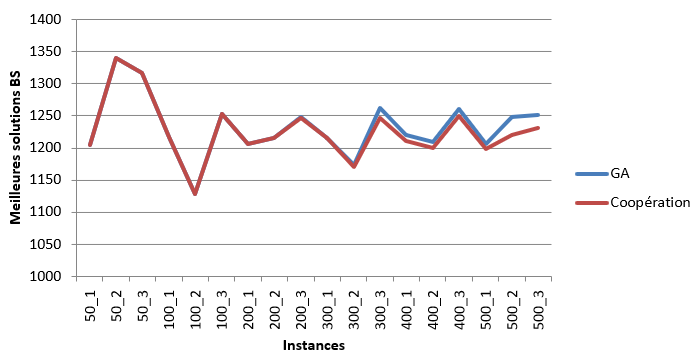
\includegraphics[width=16cm,height=7cm]{Chap5/4.png}
	\caption{Diagrammes d’exécutions de la méthode GA et la méthode coopérative}
	\label{fig:DEMGAMC}
\end{figure}


\end{enumerate}


\subsubsection{Comparaison de la méthode coopérative avec les travaux liés au DTP}
Afin de monter l’efficacité et la robustesse de notre approche coopérative, Nous l’avons comparé à deux techniques méta-heuristiques basées sur un essaim dans la littérature, à savoir ACO\_DT [55] et ABC\_DT [54], et une autre méta-heuristique SSGA \cite{sundar2014steady} .


\begin{enumerate}[label=\alph*)]
	\item \textbf{Comparaison de  la méthode coopérative avec ABC\_DTP}\\
	Dans le tableau V.5 notre méthode de coopération est meilleure sur 5 instances et similaire pour 11 instances sur 18 instances. En termes de solution moyenne, on remarque que la coopération est meilleure sur 8 instances, de moindre qualité pour 8 autres instances et est similaire pour 2 instances.
	
\begin{table}[H]
	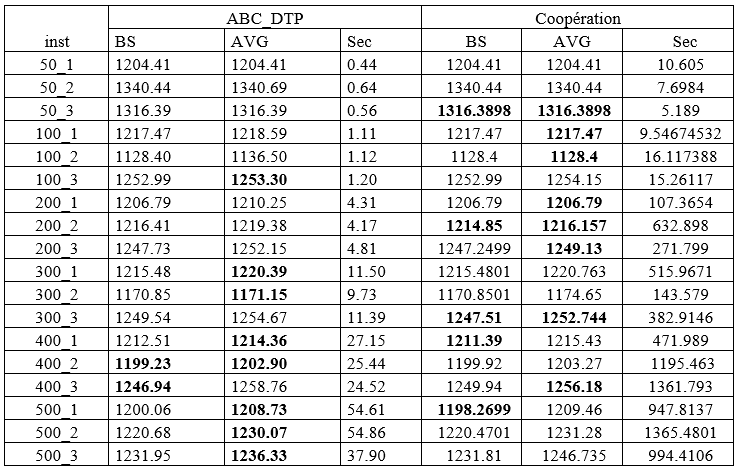
\includegraphics[width=15cm,height=8cm]{Chap5/t5.png}
	\caption{Résultats d’exécutions de ABC\_DTP et la méthode de coopération}
	\label{tab:5}
\end{table}

	\item \textbf{Comparaison de  la méthode coopérative avec ACO\_DT}\\
	D’après le tableau \ref{tab:6}, il est bien clair que la méthode de coopération est la meilleure technique en terme de la meilleure solution ainsi que la qualité moyenne de la solution. La méthode de coopération a pu générer un BS de meilleure qualité que celui d’ACO\_DT pour la plupart des instances (huit instances) et une solution de moindre qualité par rapport à celle d’ACO\_DT. Pour le reste des instances les résultats sont similaires pour les deux techniques. Concernant les moyennes des solutions obtenues (AVG), la coopération donne de meilleurs résultats que ACO\_DT dans 13 instances, et fournit une solution de moindre qualité dans une seule instance. Les résultats sont similaires pour le reste des instances (6 instances).
	
\begin{table}[H]
	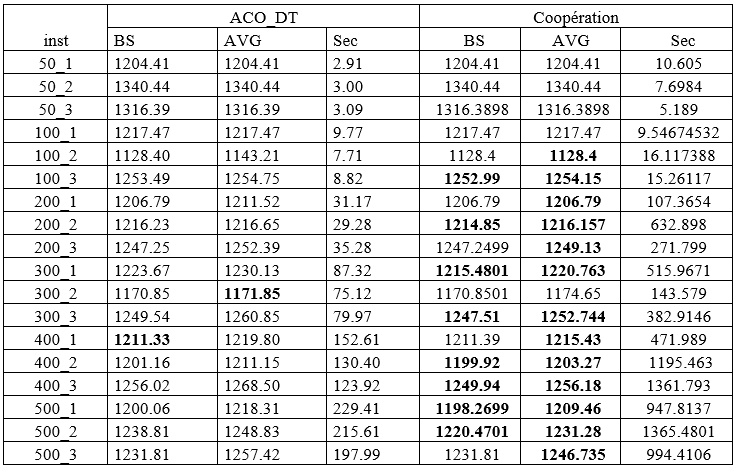
\includegraphics[width=15cm,height=8cm]{Chap5/t6.png}
	\caption{Résultats d'exécutions d'ACO\_DT et la méthode de coopération}
	\label{tab:6}
\end{table}


	\item \textbf{Comparaison de  la méthode coopérative avec SSGA}\\
	Comme le tableau \ref{tab:7} le montre, parmi les quatre  instances, la meilleure solution (BS) obtenue par la coopération est similaire à celle obtenue par SSGA dans 11 instances et est moins bonne que le BS trouvé par SSGA dans une seule instance (400\_3).
	
Concernant les moyennes des solutions (AVG), celles obtenues par la coopération sont similaires à celles obtenues par SSGA dans deux instances (50\_2 et 300\_2) et sont de moindre qualité par rapport à SSGA dans une seule instance (100\_3).

	
\begin{table}[H]
	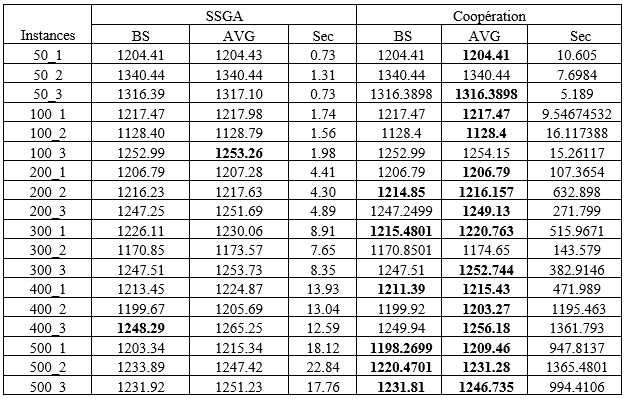
\includegraphics[width=15cm,height=8cm]{Chap5/t7.png}
	\caption{Résultats d’exécutions de SSGA et la méthode de coopération}
	\label{tab:7}
\end{table}

\end{enumerate}


\subsection{Analyse graphique}

\subsubsection{Étude comparative entre les différentes approches sur les meilleures solutions (BS) }

La Figure \ref{fig:DEAP} représente graphiquement les valeurs des différentes BS obtenues
par les méta-heuristiques  ACO\_DT, BBO, GA et la méthode coopérative, pour les 18 instances. On constate que les courbes présentent la même allure pour les instances de complexité moyenne. De plus, pour les instances de 300\_2 à 500\_3, l’approche de coopération  donne des résultats avec un coût inferieur à celui des autres approches. Chose qui prouve l’efficacité de la méthode coopérative.

\begin{figure}[H]
	\centering
	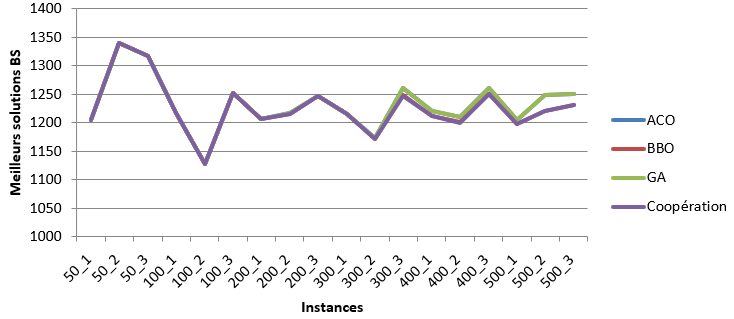
\includegraphics[width=16cm,height=7cm]{Chap5/5.png}
	\caption{Diagrammes d’exécutions des approches proposées}
	\label{fig:DEAP}
\end{figure}



\subsubsection{Comparaison de la qualité moyenne des solutions (AVG) de l’approche coopérative  et des autres approches}

La Figure \ref{fig:DQMSAP} porte sur la qualité moyenne des solutions (AVG) issues de 20 exécutions des différents algorithmes pour l’ensemble des 18 instances. On observe
que les valeurs résultantes de l’approche coopérative avoisinent celles de ACO, BBO  et GA et il est clairement aperçu que pour les grandes instances  la coopération donne de bien meilleurs résultats que les autres approches. Ceci prouve que l’approche de coopération proposée  s'adapte bien pour les grandes instances du problème. 


\begin{figure}[H]
	\centering
	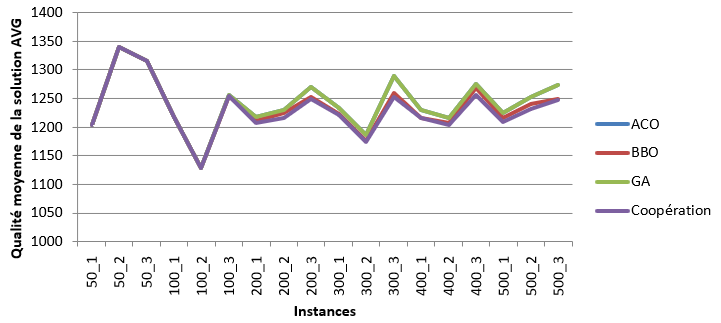
\includegraphics[width=16cm,height=7cm]{Chap5/6.png}
	\caption{Diagrammes de la Qualité moyenne de la solution AVG de des approches proposées}
	\label{fig:DQMSAP}
\end{figure}


\section{Conclusion}
A travers ce dernier chapitre, nous avons étudié les résultats expérimentaux de l’approche proposée et les avons comparées selon quelques paramètres de performances (BS,AVG), avec d’autres travaux élaborés pour la résolution du problème de l’arbre dominant. Dans l’ensemble, les approches que nous avons proposées se sont  avéré efficace en offrant de bons résultats malgré la constatation de quelques dégradations de qualité qui peut se justifier par la nature stochastique des méta-heuristiques.




\addcontentsline{toc}{chapter}{\numberline{}Conclusion général}

\begin{center}
	\LARGE\textbf{Conclusion général}
\end{center}


Les travaux présentés dans ce projet de fin d’études traitent le fameux problème de l’arbre dominant qui est un des problèmes les plus traités dans le domaine de l'optimisation combinatoire.

Ce problème est apparu à l’époque où les Réseaux de Capteurs Sans Fils (RCSF) ont connu un  grand développement ce qui leur a permis d’occuper une place très importante dans le monde de la recherche scientifique.  En effet, il est né lors de de l’ apparition de la contrainte d’énergie  qui représente un inconvénient majeur dans les RCSFs. Les plus grands taux de la consommation d’énergie ont lieu lors de la transmission des données.

Une des solutions consiste à fournir une ossature pour l’optimisation du routage des données permettant ainsi une économie d’énergie. Ceci revient à rechercher un arbre dominant de poids minimal.

L’objectif principal de notre projet de fin d’études est de proposer une méthode pour la résolution du problème de l’arbre dominant. Afin d’arriver à bout de notre solution, une étude des différentes techniques d’optimisation combinatoire a été nécessaire, ainsi qu’une étude approfondie des travaux élaborés dans le même but. Ce qui nous a permis  d'adapter quelques méta-heuristiques inspirées de travaux antécédents.

Nous avons également mis en œuvre une nouvelle approche nommé l’approche coopérative, qui consiste à faire coopérer plusieurs maté-heuristiques esclaves soumises au contrôle d'une méta-heuristique maître. Malgré la difficulté du problème traité, ce fut véritablement une expérience fructueuse qui nous a ouvert les portes vers de nouveaux horizons. Pour conclure, nous avons réussi à mener notre projet à terme. L’application réalisée, nous a permis, comme prouvé dans les différents graphes d’atteindre des résultats très proches de ceux des travaux antérieurs et d’améliorer la majorité. 

En guise de perspectives, nous envisageons d’intégrer un mécanisme d’adaptation des paramètres qui permettra de guider le comportement du processus de recherche en fonction d’indicateurs collectés au cours de l’exécution, ce qui ouvre par la suite une nouvelle fenêtre pour la recherche. Nous aimerions aussi, adapter l’approche proposée à d’autres problèmes similaires.



\bibliographystyle{IEEEtran}
\bibliography{General/References}




\thispagestyle{empty}

\LARGE\textbf{Résumé}

\Large{}
\end{document}

